\subsection{Matrix notation} \label{sec:mat_pol_intro}
In this section we cast the relation introduced in Sec.~\ref{sec:pol-primer} in matrix notation\footnote{While we work with the matrix and vector sizes given in terms of Healpix pixelization parameter $\rm N_{\rm pix}$, all the relations are equally valid in the continuum limit attained by allowing $\rm N_{\rm pix}\rightarrow \infty$}. This representation will make transparent the derivation of the real space operators we discuss in the following sections. We adopt a convention in which real space quantities are denoted by bar-ed variable while those in harmonic space are denoted by tilde-ed variables.\\
We begin by introducing the matrices encoding the spin spherical harmonic basis vectors,
%
\beq
_sB= \bmat _{+s}Y & 0 \\ 0 & _{-s}Y \emat _{2 \rm N_{\rm pix} \times 2 \rm N_{\rm alms}} \,,
\eeq
%
where $s$ denotes the spin of the basis functions. For this work we will only be working with cases $s \in [0,2]$. In this notation, each column can be mapped to a specific harmonic basis function marked by the pair of indices:$(\ell,m)$ and each row maps to a specific position on the sphere. Note that this matrix is in general not a square matrix. Generally the number of columns is determined by the scheme used to discretely represent the sphere and the number of rows is set by the number of basis functions of interest (often determined the band limit).

We now define the different data vectors and their representation in real and harmonic space as follows,
%
\beqrys
\bar{S} &=& \bmat E \\ B  \emat_{2 \rm N_{\rm pix} \times 1} ~~~~;~~ \bar{X} = \bmat _{+2}X \\ _{-2}X \emat_{2 \rm N_{\rm pix} \times 1} ~~;~~\bar{P} =\fqu_{\tiny {2 \rm N_{\rm pix} \times 1}} \,, \\
\tilde{S} &=& \bmat a^{E} \\ a^{B} \emat _{2 \rm N_{\rm alms} \times 1}  ~~; ~~ \tilde{X} = \bmat _{+2} \tilde{X} \\ _{-2} \tilde{X} \emat_{2 \rm N_{\rm alms} \times 1} \,.
\eeqrys
%
The different symbols have the same meaning as that discussed in \sec{sec:pol-primer}, except that the subscript $_{\ell m}$ for the spherical harmonic coefficients of expansion is suppressed to avoid clutter in notation.

Next we define the operators which govern the transformations between different representations of the polarization field as follows,
%
\beqrys
\bar T &=& \qutox_{2 \rm N_{\rm pix} \times 2 \rm N_{\rm pix}} ~~;~~ \bar T^{-1} = \frac{1}{2} \bar T^{\dagger} \,, \\
\tilde T &=& -\qutox_{2 \rm N_{\rm alms} \times 2 \rm N_{\rm alms}} ~~;~~ \tilde T^{-1} = \frac{1}{2} \tilde T^{\dagger} \,. 
\eeqrys
%
Using the data vectors and the all the operators defined in this section we now write down, in compact notation, the forward and inverse relations between different representations of the polarization field as follows,
%
\beqrys \label{eq:pol_data_relns}
\bar{X} &=& \bar T * \bar{P} ~~;~~\bar{P} = \frac{1}{2} \bar T^{\dagger} * \bar{X} \,, \\
\bar X &=&  {_2B} * \tilde X  ~~;~~ \tilde X ={_2B}^{\dagger} * \bar X  \,, \\
\tilde{X} &=& \tilde T * \tilde{S} ~~;~~ \tilde{S} = \frac{1}{2}\tilde T^{\dagger} * \tilde{X} \,.\\ 
\bar S &=&  {_0B} * \tilde S ~~;~~  \tilde S =  {_0B}^{\dagger} * \bar S \,.
%\tilde X &=&  {_2B}^{\dagger} * \bar X ~~;~~ \tilde{X} = \tilde T * \tilde{S} \,, \\
%\bar{S} &=& {_0B}*\tilde S ~~;~~ \tilde{S} = \frac{1}{2}\tilde T^{\dagger} * \tilde{X} \,.\\
%\bar{X} &=& \bar T * \bar{P} ~~;~~ \tilde{X} = \tilde T * \tilde{S} \,, \\
%\bar{P} &=& \frac{1}{2} \bar T^{\dagger} * \bar{X} ~~;~~ \tilde{S} = \frac{1}{2}\tilde T^{\dagger} * \tilde{X} \,. \\
\eeqrys
%
Next we introduce the harmonic space operators, which project the harmonic space data vector to E or B subspace,
%
\beqrys
\tilde O_E &=& \bmat \mathbb{1} & \mathbb{0} \\ \mathbb{0} & \mathbb{0} \emat _{2 \rm N_{\rm alms} \times 2 \rm N_{\rm alms} }   ~~;~~ \tilde S_E = \tilde O_E* \tilde S \,,\\
\tilde O_B &=& \bmat \mathbb{0} & \mathbb{0} \\ \mathbb{0} & \mathbb{1} \emat _{2 \rm N_{\rm alms} \times 2 \rm N_{\rm alms} } ~~; ~~ \tilde S_B = \tilde O_B *\tilde S \,.
\eeqrys
%
Note that these harmonic space matrices are idempotent, orthogonal to each other and their sum is an identity matrix as can be explicitly seen via the following relations, 
%
\beqrys\label{eq:eb_har_proj}
\tilde O_E * \tilde O_E&=& \tilde O_E ~~;~~  \tilde O_B * \tilde O_B= \tilde O_B \,,\\
 \tilde O_E * \tilde O_B&=& \mathbb{0} \,, \\
 \tilde O_E + \tilde O_B&=& \mathbb{1} \,.
\eeqrys
%
Here it is important to note that these relations are exact in harmonic space.  \revisit{In the following sections our aim is to derive real space analogues of these harmonic space operators. }
%%%%%%%%%%%%%%%%%%%%%%%%%%%%%%%%%%%
\section{Real space operators} \label{sec:real_space_operators}
In this section we derive the real space operators which translate the Stokes parameters Q \& U to E \& B fields and vice versa. We also derive real space operators for directly(without first evaluating the E \& B field themselves) decomposing the Stokes  parameters Q \& U in to Stokes parameters that correspond to the E \& B fields respectively. We extensively make use of the matrix notation introduces in \sec{sec:mat_pol_intro} for these derivations.

All the results are most conveniently expressed as functions of the Euler angles  $\alpha, ~\beta~\&~ \gamma$ on the sphere. Generically, the Euler angles define the rotations that transforms the local cartesian coordinate system defined at the sphere position $\hat{n}_i \equiv (\theta_i,\phi_i)$ such that it aligns with the local cartesian coordinate system at the location $\hat{n}_j \equiv (\theta_j,\phi_j)$ \cite{varshalovich}. The Euler angles can be evaluated as the following functions of the angular coordinates of the points $\hat{n}_i \equiv (\theta_i , \phi_i)$ and $\hat{n}_j \equiv (\theta_j, \phi_j)$,
%
\beqrys \label{eq:fn_euler}
\cos(\beta) &=& \sin(\theta_i)\sin(\theta_j) \cos(\phi_i -\phi_j) + \cos(\theta_i)\cos(\theta_j) \,,\\
\tan(\alpha) &=& \frac{\sin(\phi_i - \phi_j) \sin(\theta_i) \sin(\theta_j)}{\cos(\theta_i) \cos(\beta) - \cos(\theta_j)} \,, \\
\tan(\gamma) &=& \frac{\sin(\phi_i - \phi_j) \sin(\theta_i) \sin(\theta_j)}{\cos(\theta_j) \cos(\beta) - \cos(\theta_i)}\,,
\eeqrys
%
where $\beta$ denotes the angular distance between the two points $\hat{n}_i$ \& $\hat{n}_j$ on the sphere, while the angles $\alpha$ \& $\gamma$ define rotations which co-align the coordinate axes of the two local coordinate systems. While evaluating the above functions we follow the convention that $\beta$ lies in the domain $[0, \pi]$ and that the angles $\alpha ~\&~ \gamma$ lie in the domain $[-\pi,\pi]$. It is important to assign the proper signs to $\alpha ~\&~ \gamma$ by duly accounting for the signs of the term in the numerator and the denominator. 
%--------------------------------------------------------
%--------------------------------------------------------
\subsection{Evaluating E \& B fields from measured Stokes parameters Q \& U}\label{sec:qu2eb}
In \sec{sec:pol-primer} we discussed how the scalar fields E \& B are derived from the Stokes parameters Q \& U. To reiterate, this process involved taking the spin harmonic transform of the complex spin-2 field $({}_{\pm2} \bar X)$, taking linear combinations of the resultant coefficients of expansion $({}_{\pm 2} \tilde X_{\ell m})$ and evaluating the forward spin-0 transform to derive the scalar E \& B fields. Here we derive the real space convolution kernels on the sphere which can be used to directly evaluate the scalar E \& B fields on the sphere.  
We use the relations given in \revisit{\eq{eq:pol_data_relns}}, to write down an equation relating the real space vector of scalars $\bar{S}^{\dagger}=[E, B]$ to the polarization vector $\bar{P}^{\dagger}=[Q, U]$ as given below,
%
\beqrys
\bar{S} &=& {_0B} *\tilde T^{-1}* {_2B^{\dagger}} *\bar T *\bar{P} = \frac{1}{2} {_0B} *\tilde T^{\dagger} {_2B^{\dagger}} *\bar T *\bar{P}   \,, \\
&=&  \bar O *\bar{P} \,.
\eeqrys
%
The explicit form of the real space operator $\bar O$ can be derived by contracting over all the matrix operators. This procedure of contracting over the operators is explicitly worked out in the following set of equations,
%
\beqrys
\bar{O} &=& \frac{1}{2} {_0B} *\tilde T^{\dagger} *{_2B^{\dagger}} *\bar T \,, \\
&=& -0.5 \yzmat{i} \qutoxd \ymatc{j} \qutox   \,, \\
&=& -0.5 \begin{bmatrix} \sum ({}_{0}Y_i ~{}_{2}Y^{T*}_j  +  {}_{0}Y_i~ {}_{-2}Y^{T*}_j) & {\rm i}  \sum ({}_{0}Y_i~ {}_{2}Y^{T*}_j - {}_{0}Y_i ~{}_{-2}Y^{T*}_j)  \\  - {\rm i} \sum  ({}_{0}Y_i {}_{2}Y^{T*}_j - {}_{0}Y_i {}_{-2}Y^{T*}_j) & \sum ({}_{0}Y_i {}_{2}Y^{T*}_j + {}_{0}Y_i {}_{-2}Y^{T*}_j)  \end{bmatrix} \,, \label{eq:qu2eb_ker_1}
\eeqrys
%
where the symbol ${}_{0}Y_i$ is used to denote the matrix ${}_{0}Y_{\hat{n}_i \times \ell m} \equiv {}_{0}Y_{\ell m}(\hat{n}_i)$, the symbol ${}_{\pm 2}Y^{T*}_j$ is used to denote the matrix ${}_{\pm 2}Y^*_{\ell m \times \hat{n}_j} \equiv {}_{\pm 2}Y^*_{\ell m}(\hat{n}_j)$ and the summation is over the multipole indices $\ell,m$. Using the conjugation properties of the spin spherical harmonic functions it can be shown that the following relation holds true,
%
\beq
 \left [\sum_{\ell m} {}_{0}Y_{\ell m}(\hat{n}_i){}_{+2}Y^*_{\ell m}(\hat{n}_j)\right]^* = \sum_{\ell m} {}_{0}Y_{\ell m}(\hat{n}_i){}_{-2}Y^*_{\ell m}(\hat{n}_j) \,.
 \eeq
 %
 where the terms on either side of the equation are those that appear in \eq{eq:qu2eb_ker_1}.
Therefore the different parts of the real space operators  are completely specified in terms of the complex function,
%
\beqrys
\mathcal{M}( \hat{n}_i, \hat{n}_j)  &=& \mathcal{M}_{r} + i \mathcal{M}_{i}  \,,\nonumber \\ 
&=&\sum_{\ell m} {{_0}Y}_{\ell m}(\hat n_i) {{_2}Y}^*_{\ell m}(\hat n_j) = \sum_{\ell} \sqrt{\frac{2\ell+1}{ 4 \pi}}{{_0Y}^*_{\ell 2}}(\beta_{ij},\alpha_{ij})\,,\\
&=&  \Big [ \cos(2 \alpha_{ij}) - i \sin(2 \alpha_{ij} ) \Big]   \sum_{\ell=\ell_{\rm min}}^{\ell_{\rm max}} {\frac{2\ell+1}{ 4 \pi}} \sqrt{\frac{(\ell-2)!}{(\ell+2)!}}P_{\ell 2} (\cos\beta_{ij}) \,, \label{eq:rad_ker_queb} \\
&=&  \Big [ \cos(2 \alpha_{ij}) - i \sin(2 \alpha_{ij} ) \Big] f(\beta_{ij},\ell_{\rm min},\ell_{\rm max}) \,, 
\eeqrys
%
where we have used the property of summation over spin spherical harmonics (see \eq{eq:sum_spin_shf}) listed in Appendix \ref{sec:ylm_mathprop}. Here we first note that this function does not depend on the Euler angle $\gamma$. This function has a part which depends only on the Euler angle $\alpha$ and this part of the function has no multipole dependence.  except the factor of 2 which arises because the polarization field is a spin-2 field. The other part of the function $f(\beta,\ell_{\rm min},\ell_{\rm max})$ depends only on the Euler angle $\beta$ and completely incorporates the multipole dependence of the function. $f(\beta,\ell_{\rm min},\ell_{\rm max})$ will be often be referred to as the radial kernel. The radial kernel is what determines the locality of the operator which translates the Stokes parameters Q \& U to the scalars E \& B.  

Finally the real space operator can be cast in this simple form,
%
\beq\label{eq:op_qu2eb}
\bar O =\bmat  -\mathcal{M}_{r} & -\mathcal{M}_{i} \\  \mathcal{M}_{i}  & -\mathcal{M}_{r} \emat_{2 N_{\rm pix} \times 2 N_{pix}} = -f(\beta_{ij},\ell_{\rm min},\ell_{\rm max})\bmat \cos(2 \alpha_{ij}) & \sin(2\alpha_{ij})\\  -\sin(2 \alpha_{ij})  & \cos(2 \alpha_{ij}) \emat \,,
\eeq
%
where i,j indices map to the location $\hat{n}_i$ and $\hat{n}_j$ on the sphere. \revisit{A similar equation for real space E \& B operators was derived in \cite{Zaldarriaga2001a}, however those results are derived for the flat sky case and do not explicitly derive the radial kernel.} \comment{Maybe a discussion on this should be in the conclusions.}

The scalar fields E \& B can now be directly derived from the measured Stokes Q \& U parameters by evaluating the following expression,
%
\beq \label{eq:qu2eb_convolution}
\bmat E_i \\ B_i  \emat= -f(\beta_{ij},\ell_{\rm min},\ell_{\rm max})\bmat \cos(2 \alpha_{ij}) & \sin(2\alpha_{ij})\\  -\sin(2 \alpha_{ij})  & \cos(2 \alpha_{ij}) \emat  \bmat Q_j \\ U_j  \emat \Delta \Omega\,,
\eeq
%
where we have used the Einstein summation convention: repeated indices are summed over. The factor $\Delta \Omega$ accounts for the finite pixel size and is important for proper normalization. \revisit{This has an elegant interpretation: to derive the E and/or B field at any given position we need to find the cosine quadrupole transform and the sine quadrupole transform of the Stokes Q \& U parameters on circles around this position, weigh the transform by the value of the function $f(\beta,\ell_{\rm min},\ell_{\rm max})$, $\beta$ being the radius of the circle and sum up the results with appropriate signs, to construct the respective scalar fields.}
\rfedit{While the azimuthal operations do not depend on the choice of basis functions, the radial kernel is completely determined by the choice of the basis functions. One can now think of constructing alternate basis functions which have different radial fall off.}
%--------------------------------------------------------
%--------------------------------------------------------
\subsection{Evaluating Stokes parameters Q \& U fields from E \& B fields}\label{sec:eb2qu}
The real space operator which translates E \& B fields to Stokes parameters Q \& U is derived using a similar procedure. The inverse operator is given by the following expression,
%
\beqry
\bar{P} &=& \bar{T}^{-1} *{_2B} *\tilde T *{_0B^{\dagger}}\bar{S} = \frac{1}{2} \bar{T}^{\dagger} *{_2B} *\tilde T *{_0B^{\dagger}}\bar{S}   \\
&=&  \bar O^{-1} *\bar{S}
\eeqry
%
We do not provide the explicit calculations here, since the real space inverse operator can be derived by contracting over all the matrix operators using a procedure nearly identical to that discussed in the previous section. The inverse operator is given by the following expression,
%
\beq
{\bar O}^{-1}=\bmat - \mathcal{M}_{r} & \mathcal{M}_{i} \\  -\mathcal{M}_{i}  & - \mathcal{M}_{r} \emat_{2 N_{\rm pix} \times 2 N_{pix}} =-f(\beta_{ij},\ell_{\rm min},\ell_{\rm max})\bmat \cos(2 \alpha_{ij}) & -\sin(2\alpha_{ij})\\  \sin(2 \alpha_{ij})  & \cos(2 \alpha_{ij}) \emat \,,
\eeq
%
where all the symbols have the same meaning as discussed in \sec{sec:qu2eb}.
Note that the kernel is different by a mere change in sign on the off-diagonals of the block matrix as compared to \eq{eq:op_qu2eb}.
We can evaluate the Stokes Q \& U parameters from the scalar E \& B  fields by evaluating the following expression,
%
\beq
\bmat Q_i \\ U_i  \emat=-f(\beta_{ij})\bmat \cos(2 \alpha_{ij}) & -\sin(2\alpha_{ij})\\  \sin(2 \alpha_{ij})  & \cos(2 \alpha_{ij}) \emat  \bmat E_j \\ B_j  \emat \Delta\Omega \,,
\eeq
%
where again the Einstein summation convention is implied and all the symbols have their usual meaning.

\comment{How does the radial kernel reduce to unity on evaluating the the operator on to its inverse ? }
%--------------------------------------------------------
%--------------------------------------------------------
\subsection{Decomposing Q \& U Stokes parameters into those corresponding to E \& B modes respectively}
The Stokes Q \& U parameters can be decomposed into the scalar modes E \& B and vice verse, as seen in the previous sections. The E \& B modes are orthogonal to each other. It is possible to decompose the Stokes Q \& U parameters into those that purely contribute to E modes and those that purely contribute to the B mode of polarization. We can only measure the total Stokes parameters which is a sum of the Stokes Q \& U corresponding to the respective scalar modes.  In this section we derive the real space operators which directly decompose the total measured Stokes Q \& U parameters to Stokes parameters corresponding to the scalar fields E \& B respectively, \textit{without ever having to evaluate the E \& B modes explicitly}. Again the procedure is analogous to that discussed in \sec{sec:qu2eb}, though the algebra is a little more involved. Here we use the harmonic space E/B projection operators $\tilde O_{E/B}$, defined in \eq{eq:eb_har_proj}, to derive the respective real space operators. It can be shown that the Stokes parameters corresponding to each scalar mode are given by the following expressions,
%
\beqry
\bar{P}_E &=&  [\bar T^{-1} * {_2B} *\tilde T * \tilde O_E* \tilde T^{-1}* {_2B^{\dagger}} *\bar T] *\bar{P}  \,, \\
&=& [\frac{1}{4} \bar T^{\dagger } * {_2B} *\tilde T * \tilde O_E* \tilde T^{\dagger} * {_2B^{\dagger}} *\bar T ]*\bar{P}  \,, \nonumber \\
&=&  \bar O_{E}*\bar{P} \,,\nonumber \\
\bar{P}_B &=&  [\bar T^{-1}* {_2B}* \tilde T* \tilde O_B* \tilde T^{-1}* {_2B^{\dagger}}* \bar T]*\bar{P}  \,, \\
&=& [\frac{1}{4} \bar T^{\dagger } * {_2B} *\tilde T * \tilde O_B* \tilde T^{\dagger} *{_2B^{\dagger}} *\bar T] *\bar{P}   \,, \nonumber\\
&=&  \bar O_{B}*\bar{P} \,. \nonumber
\eeqry
%
We contract over all the matrix operators to arrive at the the real space operators. On simplification it can be shows that the real space operator takes up the following form,
%
\beq
\bar O_{E/B} = 0.5 \bmat \mathcal{I}_{r} \pm \mathcal{D}_{r} & -\mathcal{I}_{i} \pm \mathcal{D}_{i} \\  -\mathcal{I}_{i} \pm \mathcal{D}_{i}  & \mathcal{I}_{r} \mp \mathcal{D}_{r} \emat_{2 N_{\rm pix} \times 2 N_{pix}} \,,\\
\eeq
where $\mathcal{I}_{r} ~\&~ \mathcal{D}_{r}$ and $\mathcal{I}_{i} ~\&~ \mathcal{D}_{i}$ are the real and complex parts of the following complex functions,
\beqry
\mathcal{I} &=& \mathcal{I}_{r} + i \mathcal{I}_{i} = \sum_{\ell m} {_2Y}_{\ell m}(\hat n_i) {_2Y}^*_{\ell m}(\hat n_j) \,, \nonumber \\
\mathcal{D}  &=& \mathcal{D}_{r} + i\mathcal{D}_{i} = \sum_{\ell m} {_2Y}_{\ell m}(\hat n_i) {_{-2}Y}^*_{\ell m}(\hat n_j) \,.\nonumber
\eeqry
%
These functions can be further simplified using the properties of spin spherical harmonics listed in Appendix~\ref{sec:ylm_mathprop}. Specifically it can be shown that these functions reduce to the following mathematical forms,
%
\beqrys \label{eq:fn_i}
\mathcal{I}(\hat{n}_i, \hat{n}_j) &=& \sum_{\ell} \sqrt{\frac{2\ell+1}{ 4 \pi}}{_2Y}_{\ell -2}(\beta_{ij}, \alpha_{ij}) ~ \rm{e}^{- i2 \gamma_{ij}} \label{eq:healpix-compatible-i} = \mathcal{I}_r + i \mathcal{I}_i \,, \\
\mathcal{I}_r + i \mathcal{I}_i &=& \Big [ \cos(2 \alpha_{ij} +  2\gamma_{ij}) - i \sin(2 \alpha_{ij} +  2 \gamma_{ij}) \Big]   _{-2}f(\beta_{ij},\ell_{\rm min},\ell_{\rm max}) \,,
\eeqrys
%
%
\beqrys \label{eq:fn_d}
\mathcal{D}(\hat{n}_i, \hat{n}_j) &=& \sum_{\ell} \sqrt{\frac{2\ell+1}{ 4 \pi}}{_2Y}_{\ell +2}(\beta_{ij}, \alpha_{ij}) ~ \rm{e}^{- i2 \gamma_{ij}} \label{eq:healpix-compatible-m} =\mathcal{D}_r + i \mathcal{D}_i \,, \\
\mathcal{D}_r + i \mathcal{D}_i &=&  \Big [ \cos(2 \alpha_{ij} - 2\gamma_{ij}) + i \sin(2 \alpha_{ij} -  2 \gamma_{ij}) \Big]   _{+2}f(\beta_{ij},\ell_{\rm min},\ell_{\rm max}) \,,
\eeqrys
%
where the functions,
%
\beq
{}_{\pm2}f(\beta,\ell_{\rm min},\ell_{\rm max}) = \sum_{\ell=\ell_{\rm min}}^{\ell_{\rm max}} \sqrt{\frac{2\ell+1}{ 4 \pi}} _{ \pm 2}{f}_{\ell}(\beta) \label{eq:f2_rad_ker}\,,
\eeq
%
can be expressed in terms of $P_{\ell}^2$ Legendre polynomials and are given by the following explicit mathematical forms,
 %
 \beqry
 _{\pm 2}f_{\ell}(\beta) &=& 2 \frac{(\ell-2)!}{(\ell+2)!}  \sqrt{\frac{2\ell +1 }{4 \pi}} \Bigg[ - P_{\ell}^{2} (\cos  \beta) \left( \frac{\ell-4}{\sin^2 \beta} + \frac{1}{2}\ell(\ell-1) \pm \frac{2 (\ell-1) \cos \beta}{\sin^2 \beta} \right) \nonumber \\ 
&+& P_{\ell-1}^2 (\cos \beta) \left( (\ell+2) \frac{\cos \beta}{\sin^2 \beta} \pm \frac{2 (\ell+2)}{ \sin^2 \beta } \right) \Bigg] \,. \label{eq:rad_ker_quequbqu}
 \eeqry
 %
Finally, the Stokes parameters corresponding to the respective scalar fields can be derived by evaluating the following expression, 
 %
\beqry
\bmat Q_i \\ U_i  \emat_{E/B} &=&0.5 \Bigg\lbrace {}_{-2}f(\beta_{ij},\ell_{\rm min},\ell_{\rm max}) \bmat \cos(2 \alpha_{ij} + 2\gamma_{ij}) & \sin(2\alpha_{ij} +2 \gamma_{ij}) \\  \sin(2\alpha_{ij} +2 \gamma_{ij})  & \cos(2 \alpha_{ij} + 2 \gamma_{ij}) \emat  \bmat Q_j \\ U_j  \emat   \\ &\pm& {}_{+2}f(\beta_{ij},\ell_{\rm min},\ell_{\rm max}) \bmat \cos(2 \alpha_{ij} - 2\gamma_{ij}) & - \sin(2\alpha_{ij} - 2 \gamma_{ij}) \\  -\sin(2\alpha_{ij} - 2 \gamma_{ij})  & - \cos(2 \alpha_{ij} - 2 \gamma_{ij}) \emat  \bmat Q_j \\ U_j  \emat \Bigg\rbrace \Delta\Omega \,,\nonumber
\eeqry
%
where all the symbols have their usual meaning.

 
\section{Visualizing the real space operators} \label{sec:visualize_operator}
We begin by evaluating the functions $f, _{+2}f ~\&~ _{-2}f $. Since these functions determine the amplitude of the convolution kernels as a function of the angular distance $\beta$ from the central pixel, we refer to them as the radial kernels. These functions have been calculated by evaluating the multipole sums in \eq{eq:rad_ker_queb} and \eq{eq:rad_ker_quequbqu} from $\ell_{\rm min}=2$ to $\ell_{\rm max}=96$. The resultant functions are depicted in \fig{fig:beta_kernel}. Note that the function $f(\beta)$, which is a part of the  real space convolution  kernel which translates the coordinate dependent Stokes Q \& U to coordinate independent scalars E \& B, has a vanishing contribution from the location of the central pixel ($\beta \rightarrow 0$). 
%
\begin{figure}[!hbt]
\centering
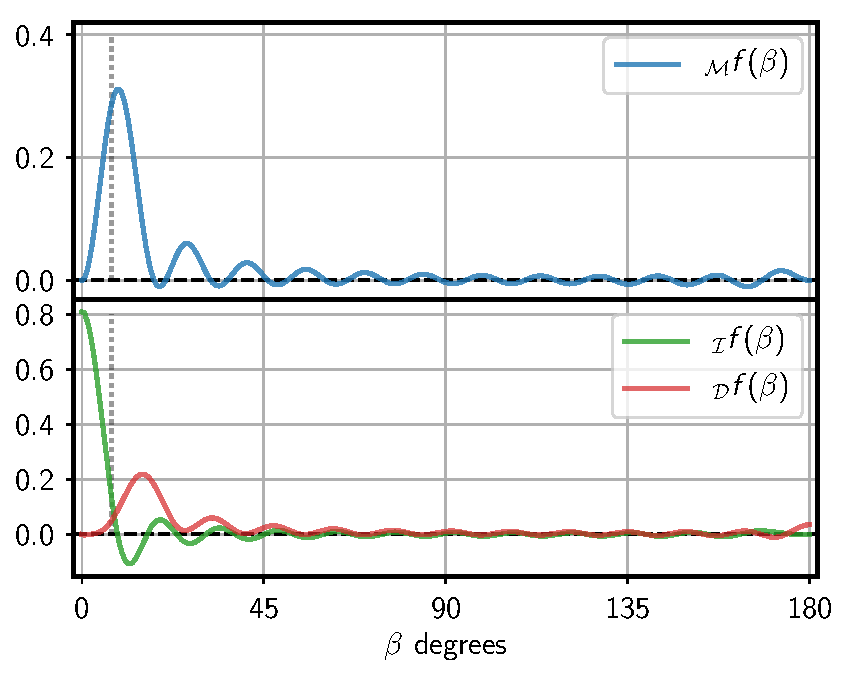
\includegraphics[width=0.8\columnwidth]{beta_kernel.pdf}
\caption{The figure depicts the radial part of the convolution kernels shown in \fig{fig:vis_kernel}. These radial function have been evaluated with the band limit fixed at $\ell_{\rm max}=96$. The vertical dashed line marks the approximate size of a NSIDE=32 Healpix pixel.}
\label{fig:beta_kernel}
\end{figure}
%
We recall that the fields E \& B are scalar and hence immune to coordinate definitions. The locally defined Stokes parameters however necessarily depend on the coordinate definition. Therefore, this nature of the radial kernel is to be expected in order for it to satisfy the requirement of the derived quantities being scalars. The functions $_{+2}f(\beta)~\&~_{-2}f(\beta)$, both contribute to the convolution kernels which decompose the Stokes parameters into those corresponding to the respective scalar modes E \& B. Note that while $_{-2}f(\beta)$ specifically contributes at the location of the central pixel, $_{+2}f(\beta)$ dominates in the neighbouring regions which are approximately at least 1 pixel away from the central pixel.

In addition to the angular distance $\beta$ from the central pixel, the convolution kernels also depend on the other Euler angles $\alpha ~\&~ \gamma$ as seen from \eq{eq:op_qu2eb}, \eq{eq:fn_i} and \eq{eq:fn_d}. We plot the real and imaginary parts of the functions $\mathcal{M}, \mathcal{D}~\&~\mathcal{I}$ at different positions on the sphere. For illustration the functions have been sampled at a very high Healpix resolution parameter of NSIDE=2048. We evaluate parts of the convolution kernels at different locations on the sphere and the results are depicted in \fig{fig:vis_kernel}. 
 %
\begin{figure}[!h] \label{fig:mixing_kernel}
\centering
\subfigure{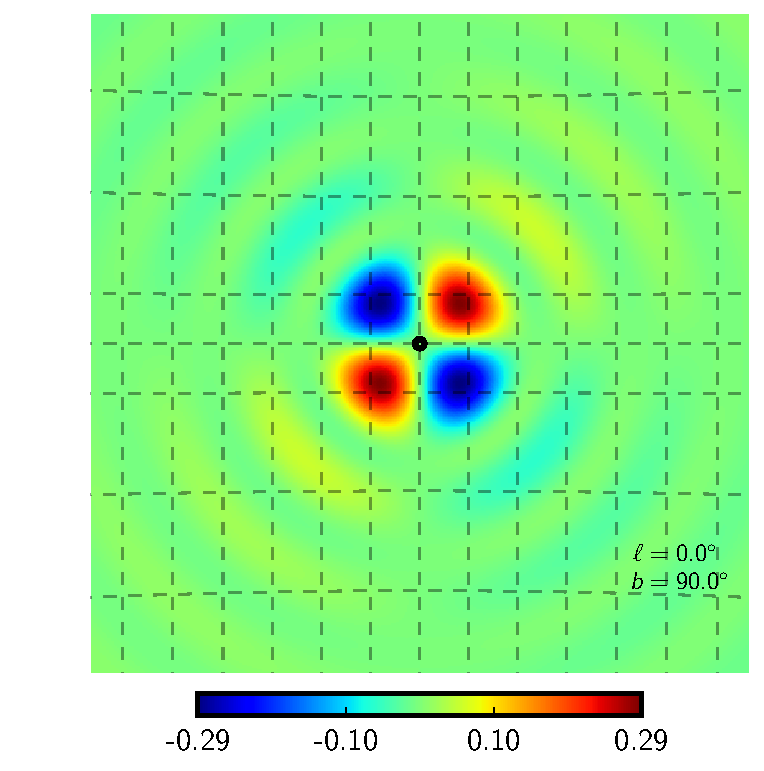
\includegraphics[width=0.16\columnwidth]{qu2eb_ker_r_lat90_lon0.pdf}}\hspace{-2mm}
\subfigure{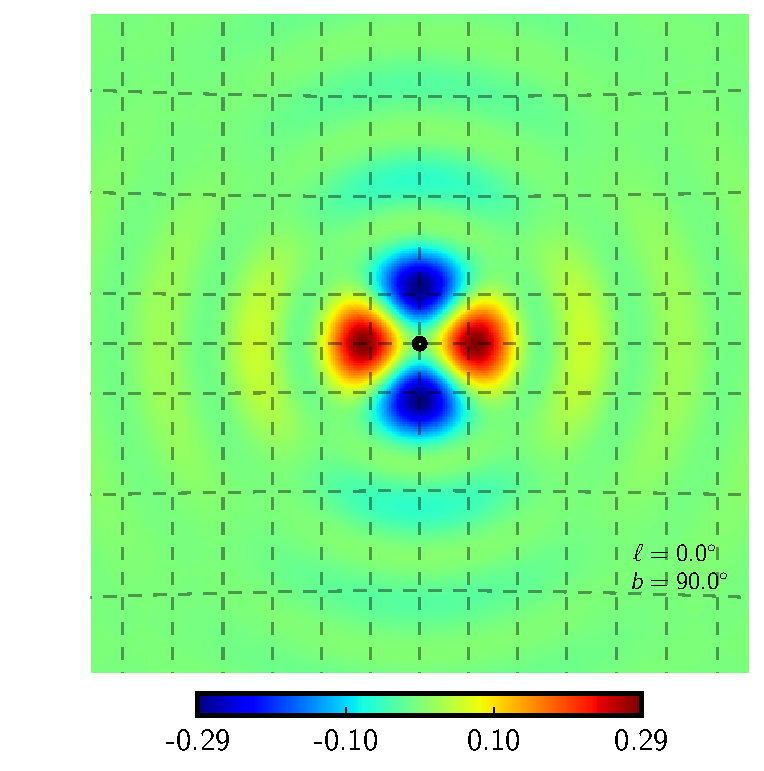
\includegraphics[width=0.16\columnwidth]{qu2eb_ker_i_lat90_lon0.pdf}}\hspace{-2mm}
\subfigure{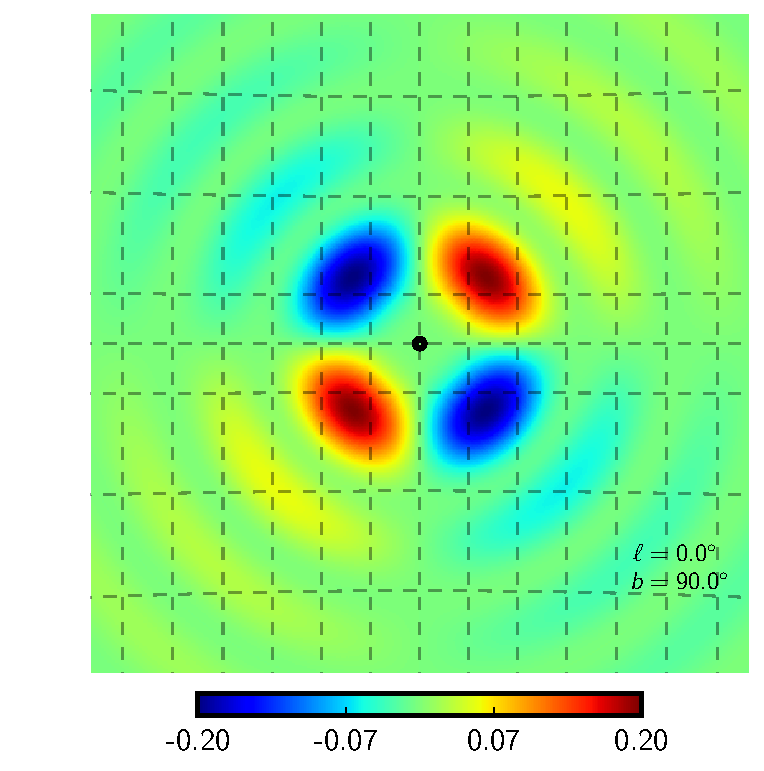
\includegraphics[width=0.16\columnwidth]{qu2ebqu_ker_r_lat90_lon0.pdf}}\hspace{-2mm}
\subfigure{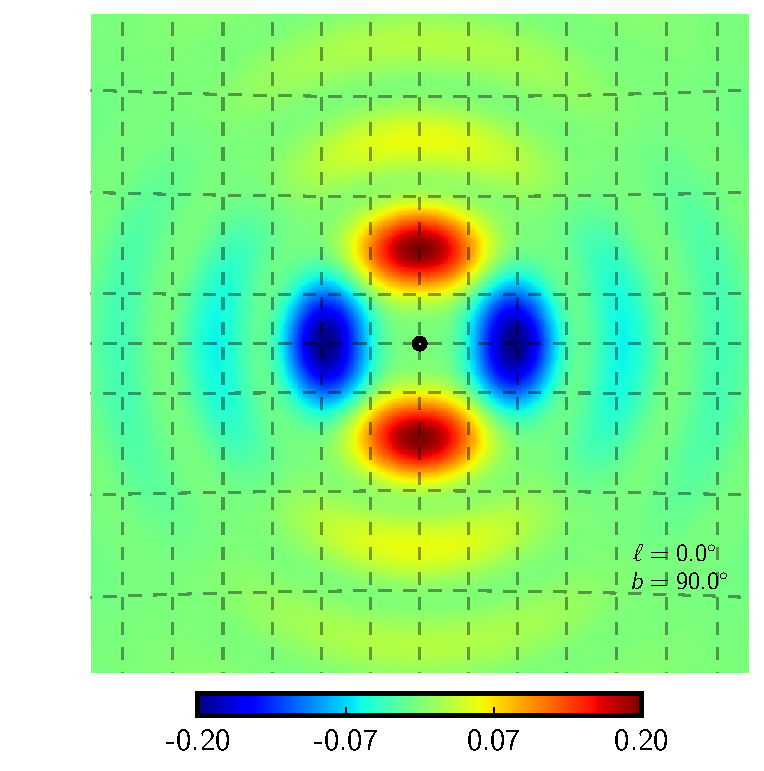
\includegraphics[width=0.16\columnwidth]{qu2ebqu_ker_i_lat90_lon0.pdf}}\hspace{-2mm}
\subfigure{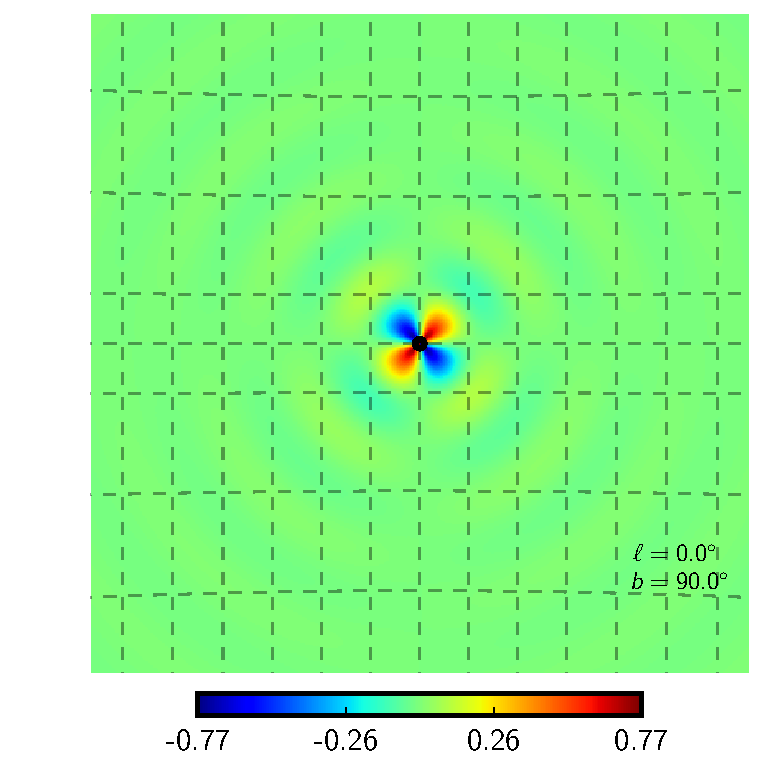
\includegraphics[width=0.16\columnwidth]{I_ker_r_lat90_lon0.pdf}}\hspace{-2mm}
\subfigure{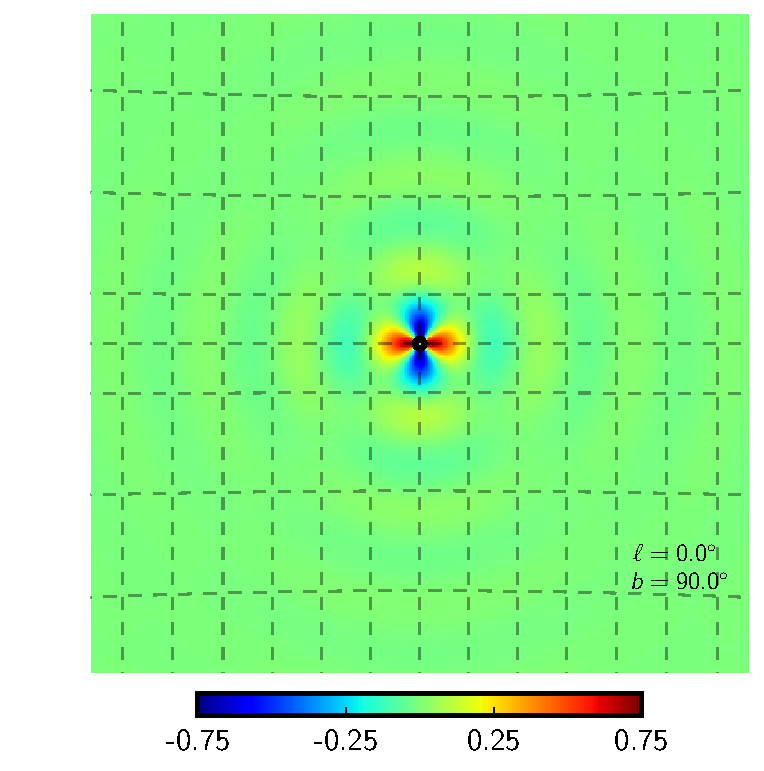
\includegraphics[width=0.16\columnwidth]{I_ker_i_lat90_lon0.pdf}}\\[-2ex]
\subfigure{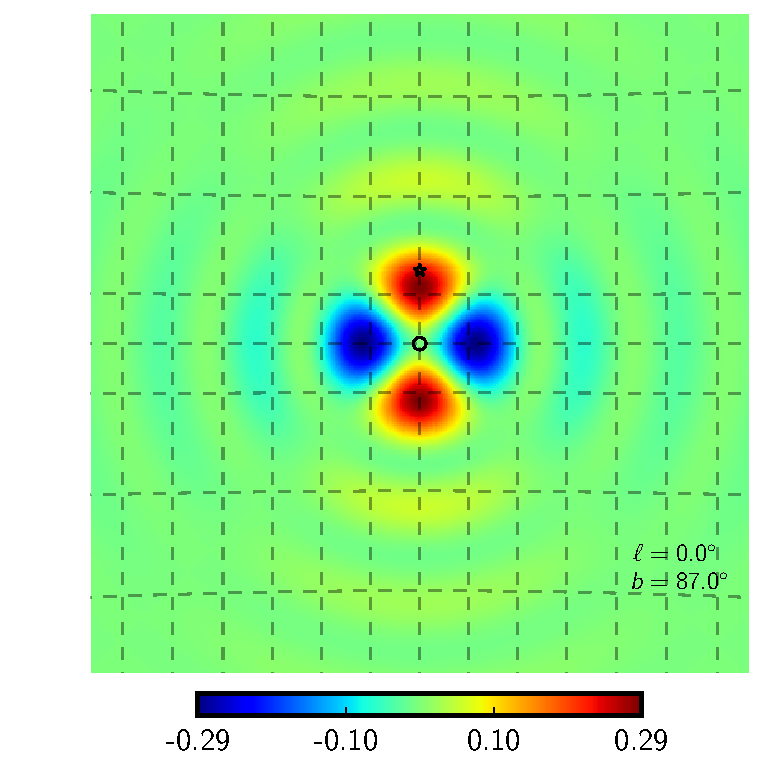
\includegraphics[width=0.16\columnwidth]{qu2eb_ker_r_lat87_lon0.pdf}}\hspace{-2mm}
\subfigure{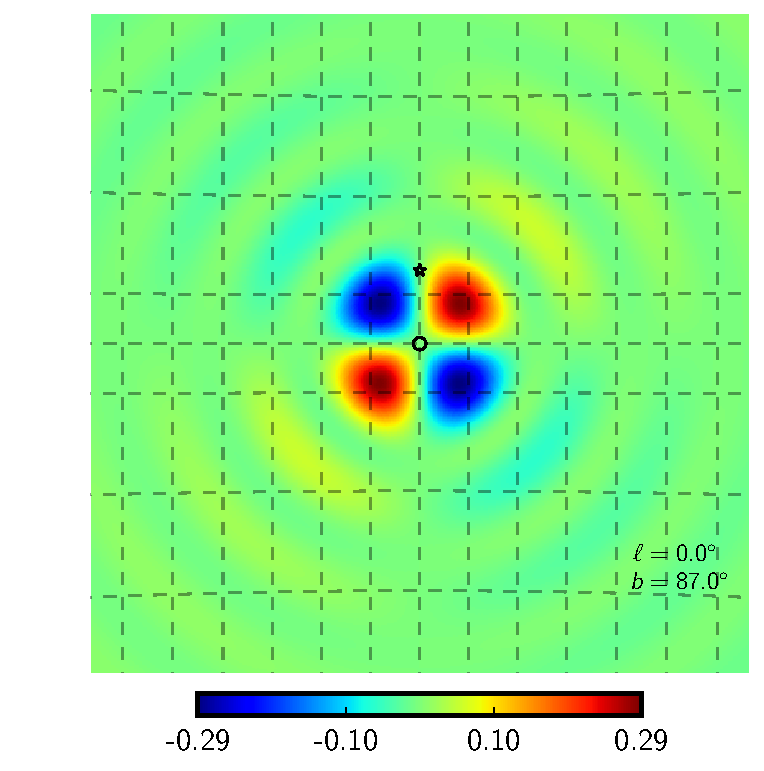
\includegraphics[width=0.16\columnwidth]{qu2eb_ker_i_lat87_lon0.pdf}}\hspace{-2mm}
\subfigure{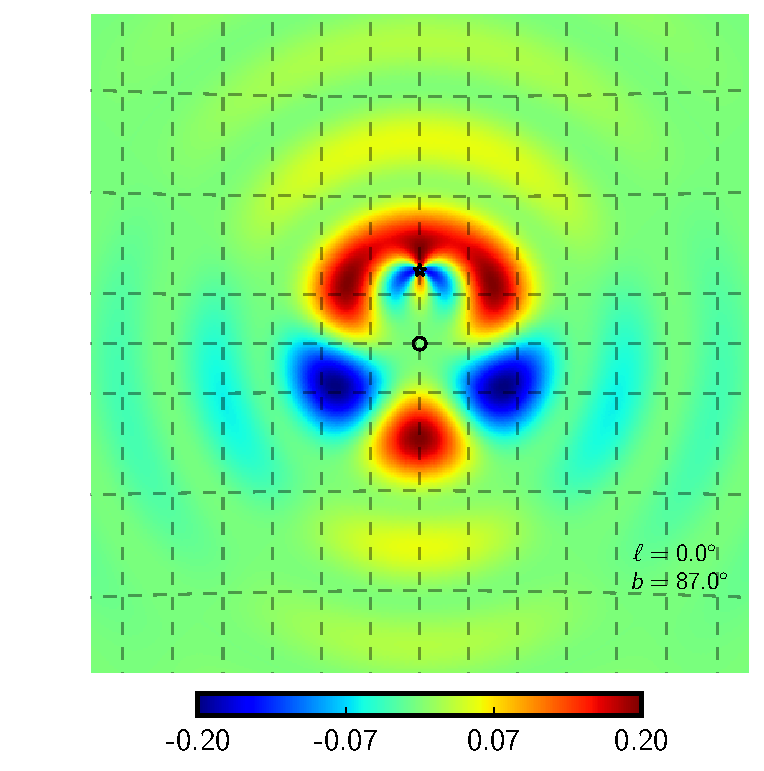
\includegraphics[width=0.16\columnwidth]{qu2ebqu_ker_r_lat87_lon0.pdf}}\hspace{-2mm}
\subfigure{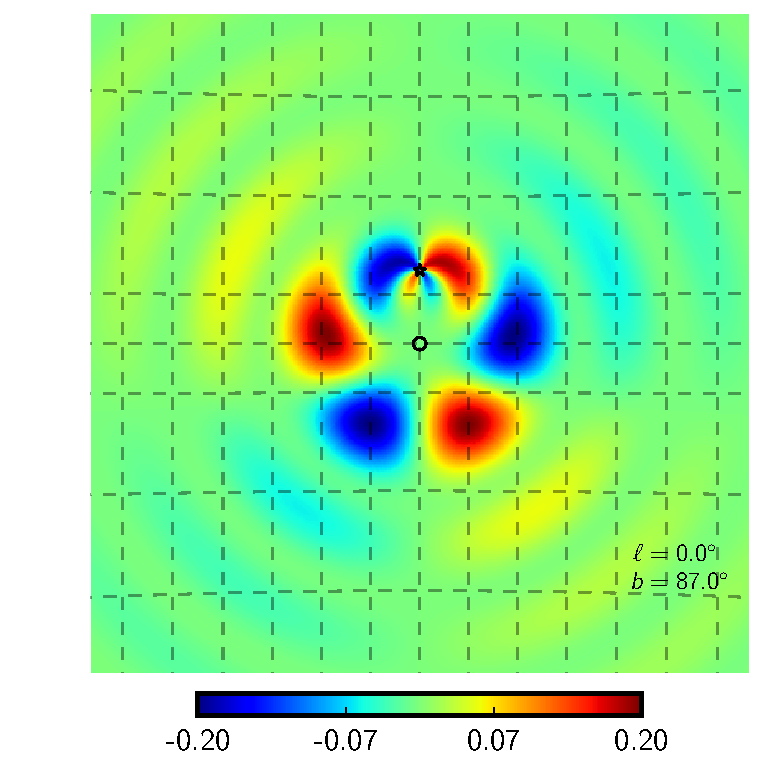
\includegraphics[width=0.16\columnwidth]{qu2ebqu_ker_i_lat87_lon0.pdf}}\hspace{-2mm}
\subfigure{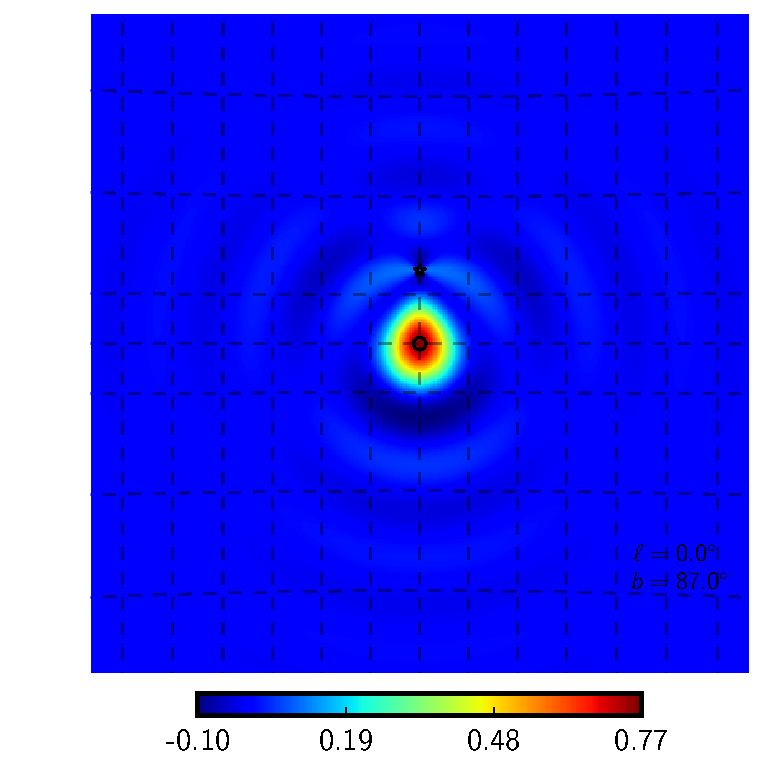
\includegraphics[width=0.16\columnwidth]{I_ker_r_lat87_lon0.pdf}}\hspace{-2mm}
\subfigure{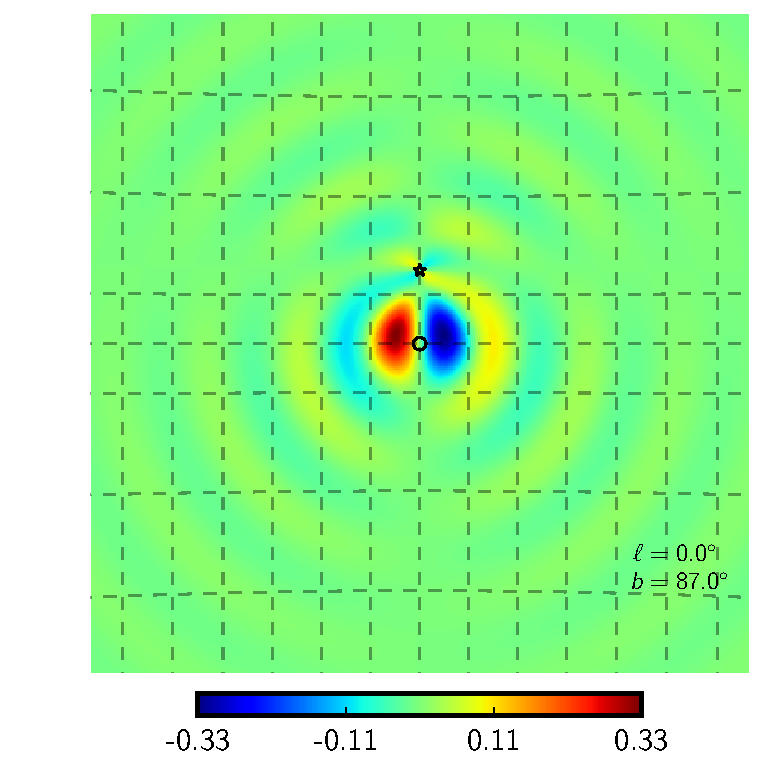
\includegraphics[width=0.16\columnwidth]{I_ker_i_lat87_lon0.pdf}}\\[-2ex]
\subfigure{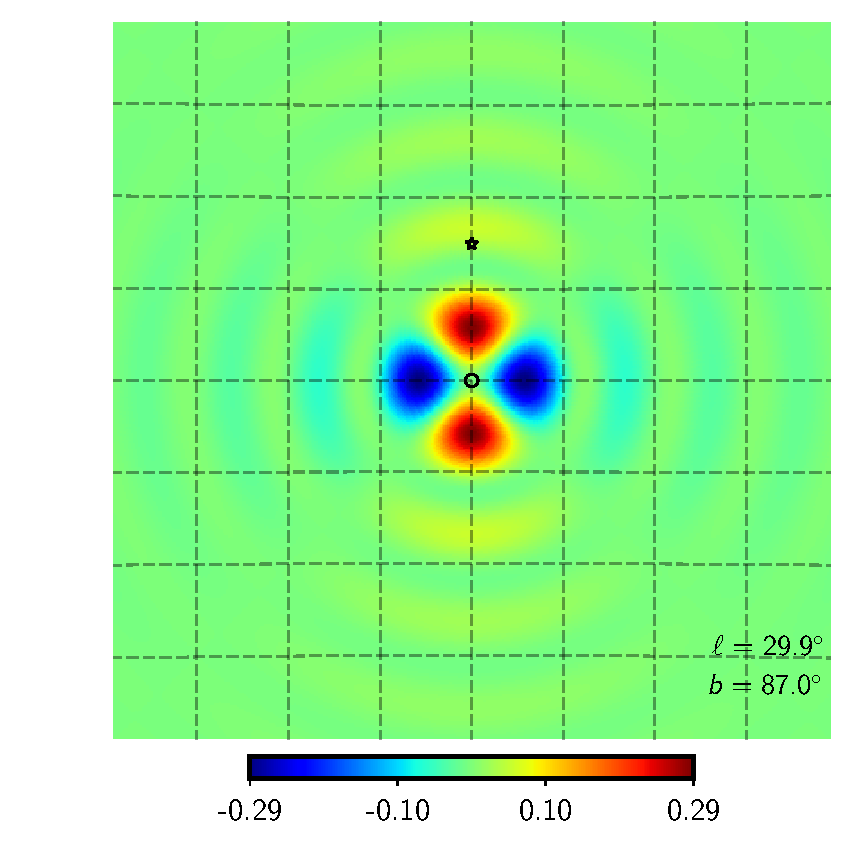
\includegraphics[width=0.16\columnwidth]{qu2eb_ker_r_lat87_lon30.pdf}}\hspace{-2mm}
\subfigure{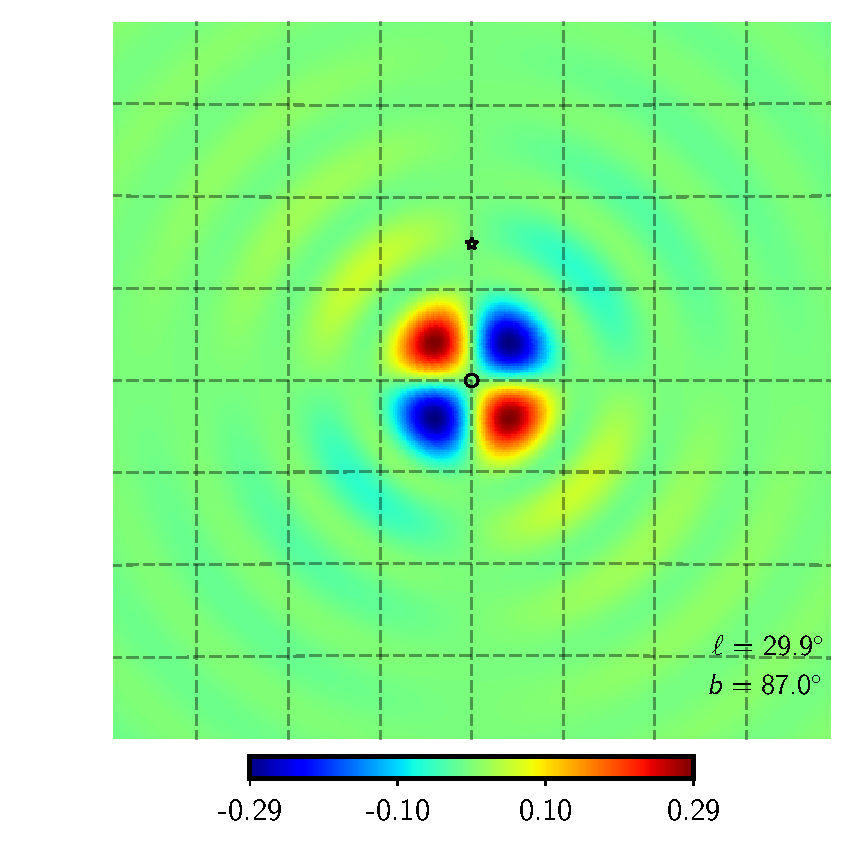
\includegraphics[width=0.16\columnwidth]{qu2eb_ker_i_lat87_lon30.pdf}}\hspace{-2mm}
\subfigure{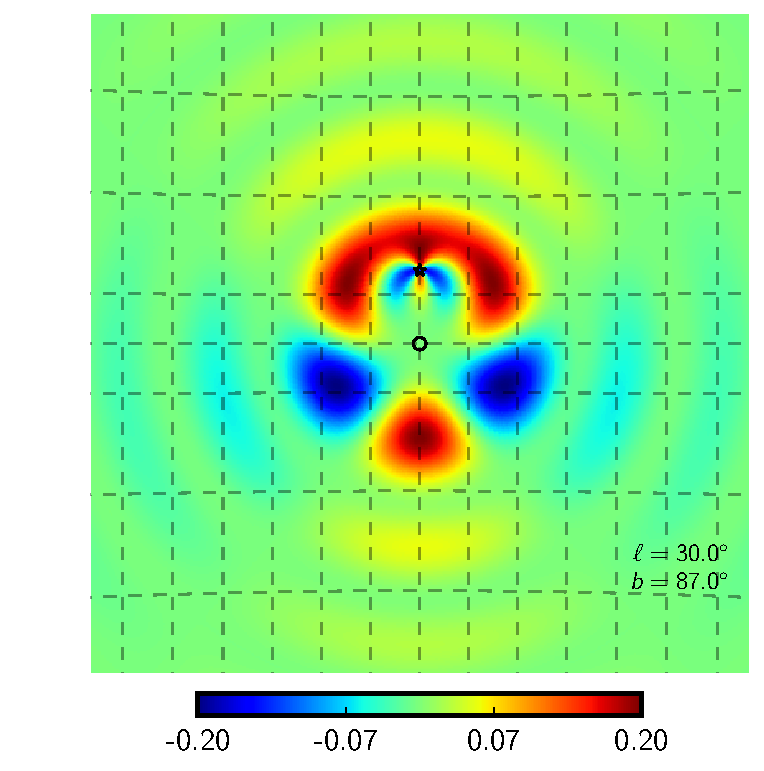
\includegraphics[width=0.16\columnwidth]{qu2ebqu_ker_r_lat87_lon30.pdf}}\hspace{-2mm}
\subfigure{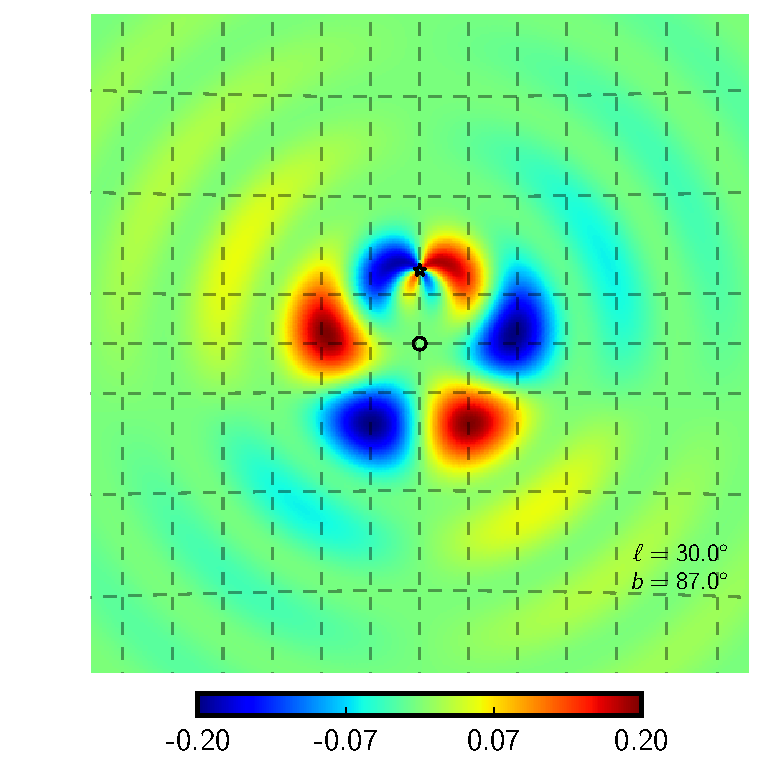
\includegraphics[width=0.16\columnwidth]{qu2ebqu_ker_i_lat87_lon30.pdf}}\hspace{-2mm}
\subfigure{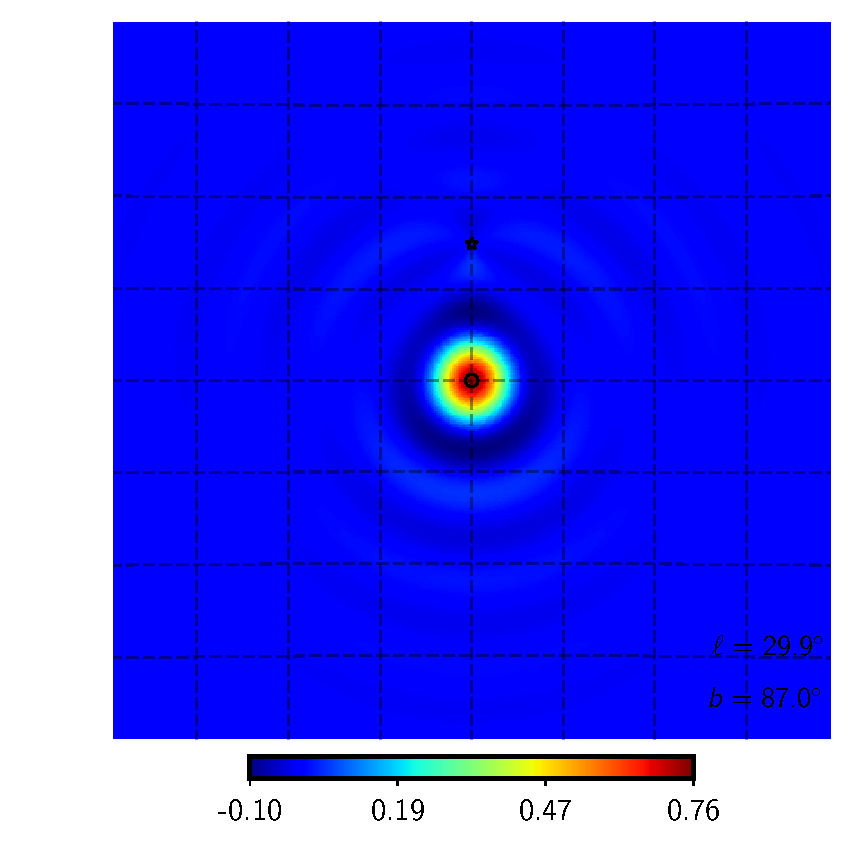
\includegraphics[width=0.16\columnwidth]{I_ker_r_lat87_lon30.pdf}}\hspace{-2mm}
\subfigure{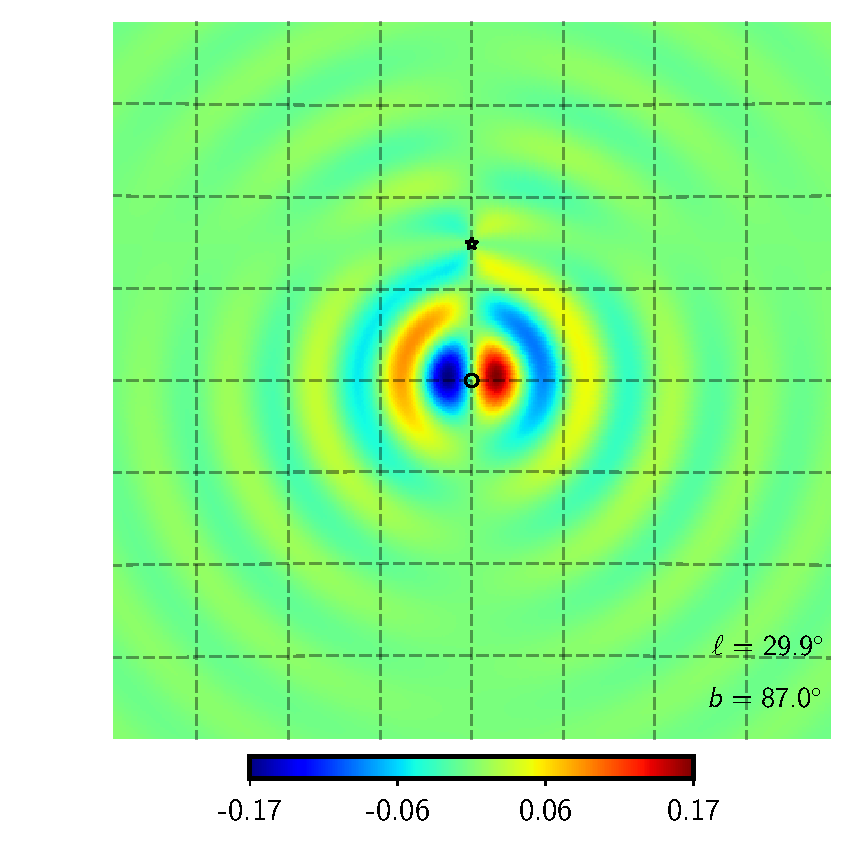
\includegraphics[width=0.16\columnwidth]{I_ker_i_lat87_lon30.pdf}}\\[-2ex]
\subfigure{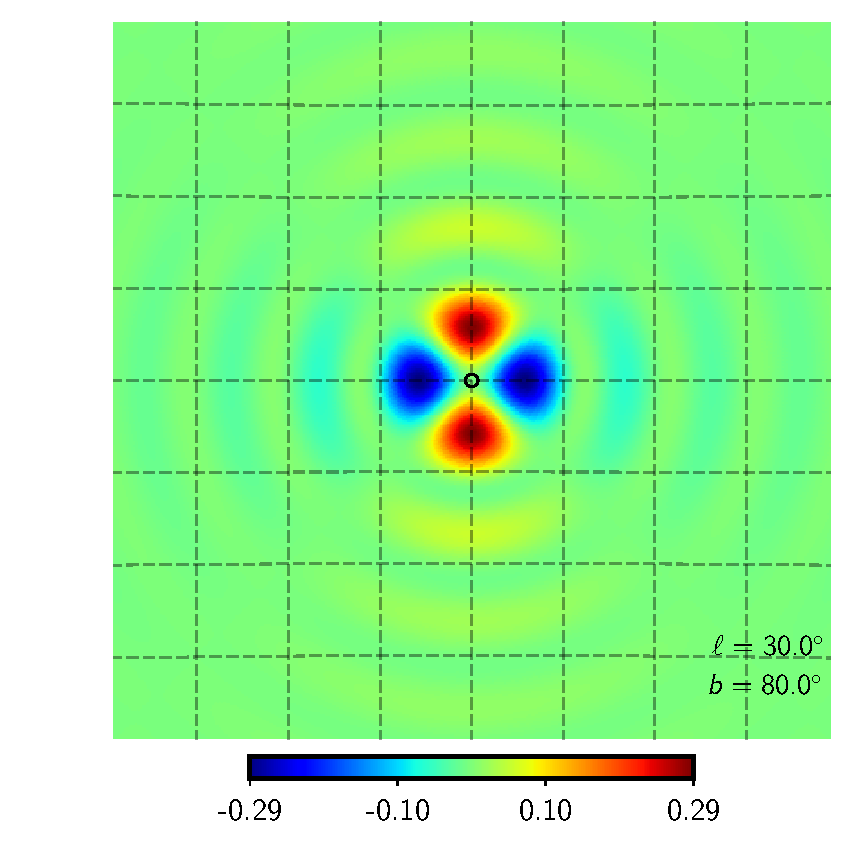
\includegraphics[width=0.16\columnwidth]{qu2eb_ker_r_lat80_lon30.pdf}}\hspace{-2mm}
\subfigure{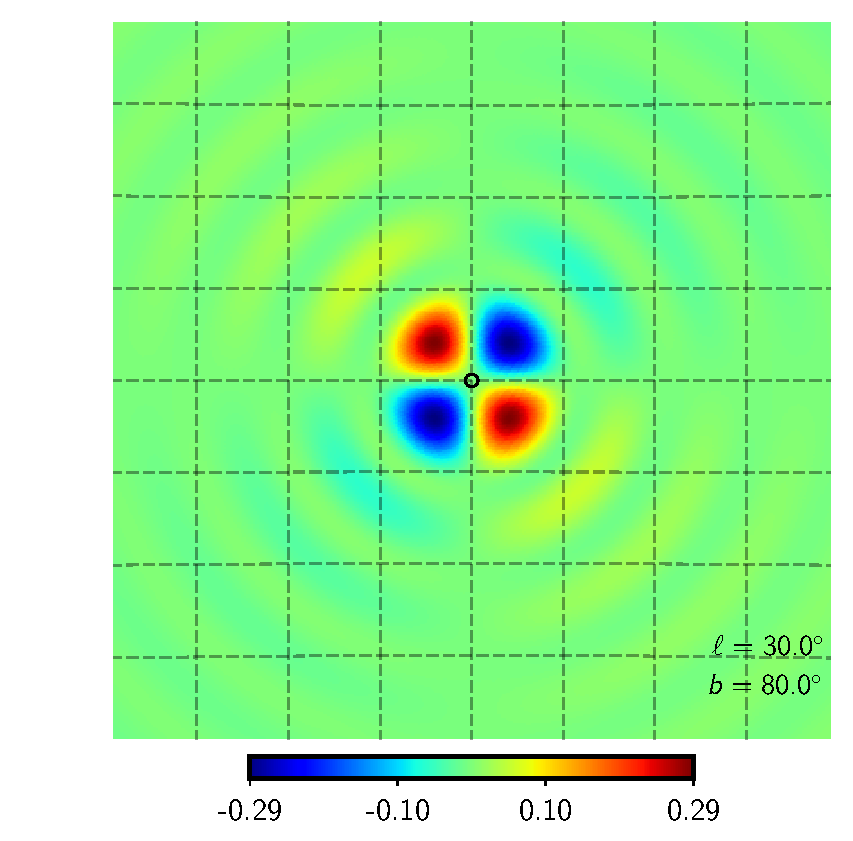
\includegraphics[width=0.16\columnwidth]{qu2eb_ker_i_lat80_lon30.pdf}}\hspace{-2mm}
\subfigure{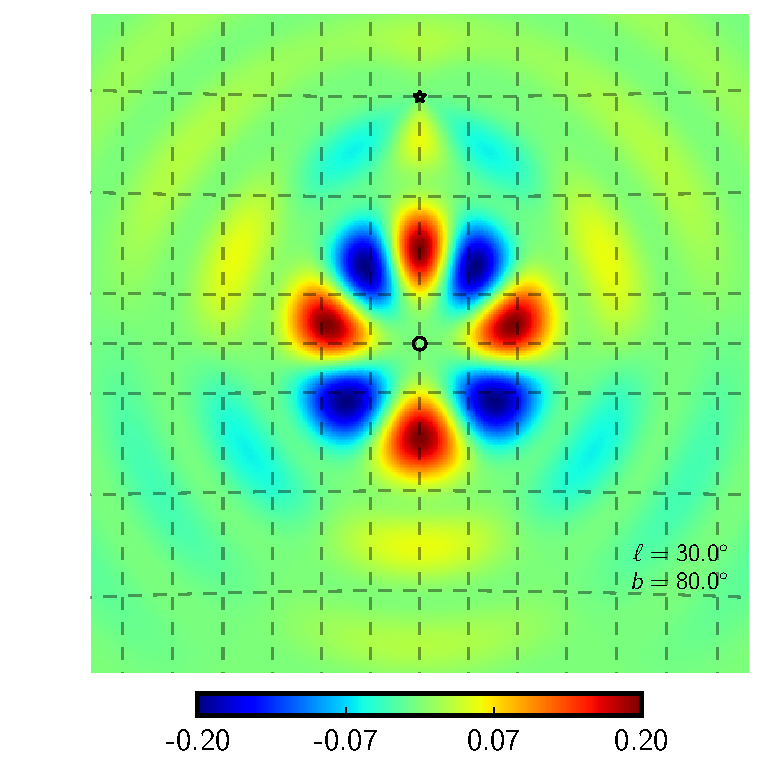
\includegraphics[width=0.16\columnwidth]{qu2ebqu_ker_r_lat80_lon30.pdf}}\hspace{-2mm}
\subfigure{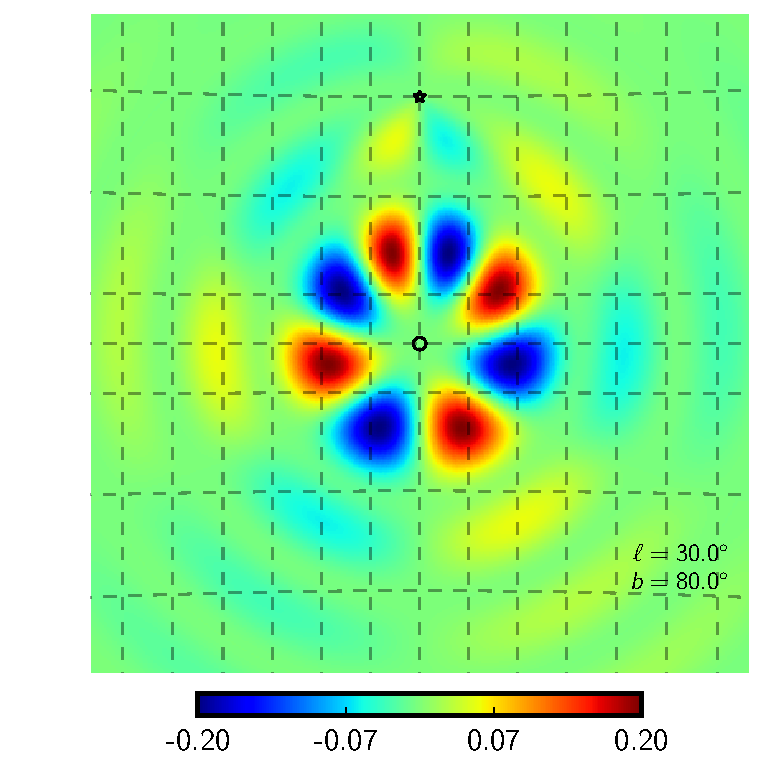
\includegraphics[width=0.16\columnwidth]{qu2ebqu_ker_i_lat80_lon30.pdf}}\hspace{-2mm}
\subfigure{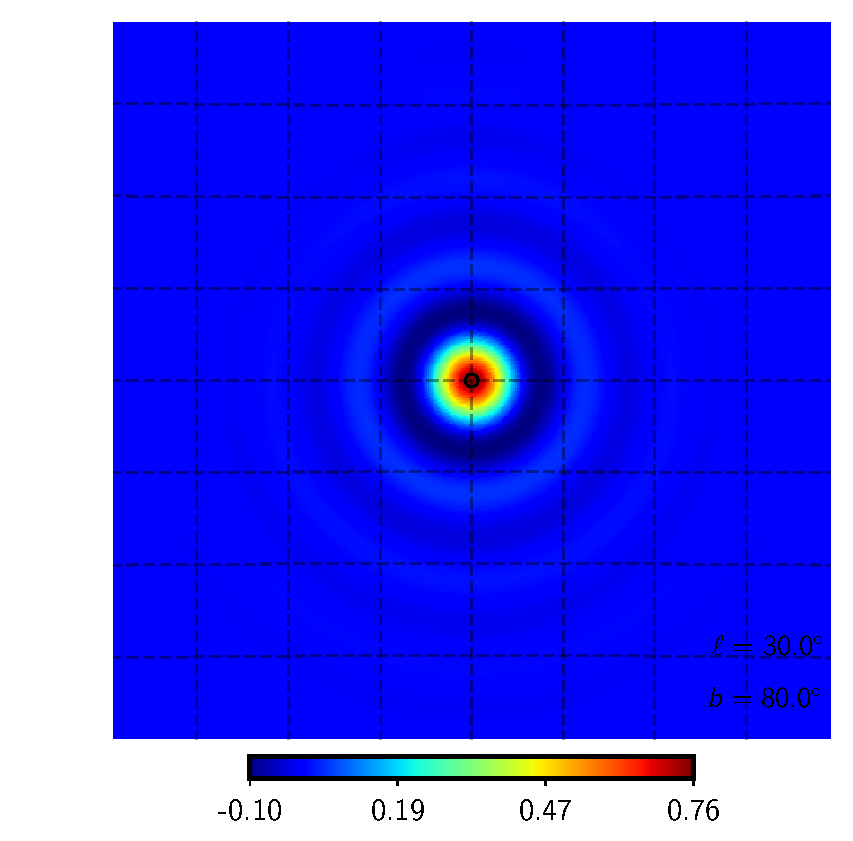
\includegraphics[width=0.16\columnwidth]{I_ker_r_lat80_lon30.pdf}}\hspace{-2mm}
\subfigure{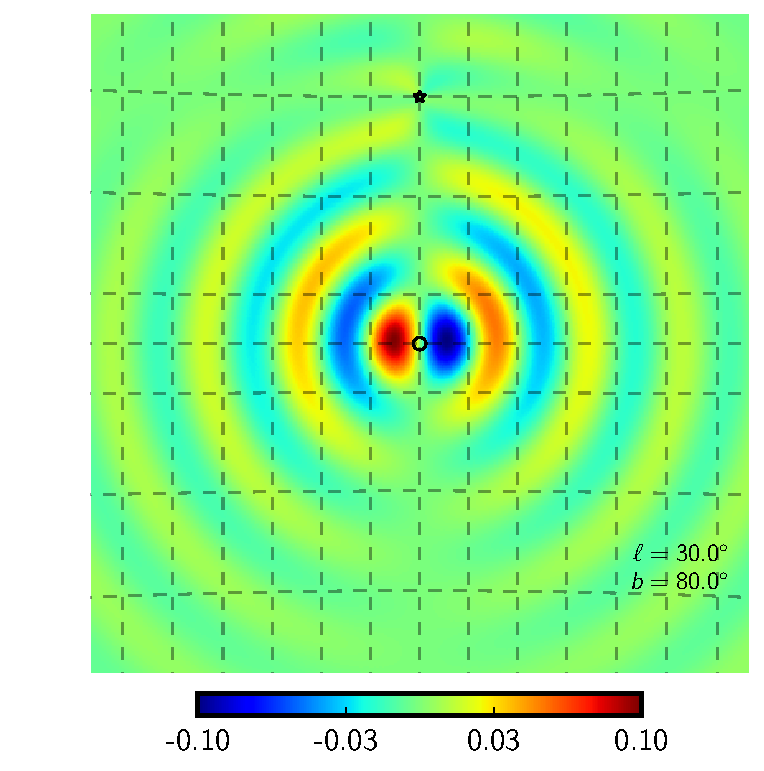
\includegraphics[width=0.16\columnwidth]{I_ker_i_lat80_lon30.pdf}}\\[-2ex]
\subfigure[$\mathcal{M}_r$]{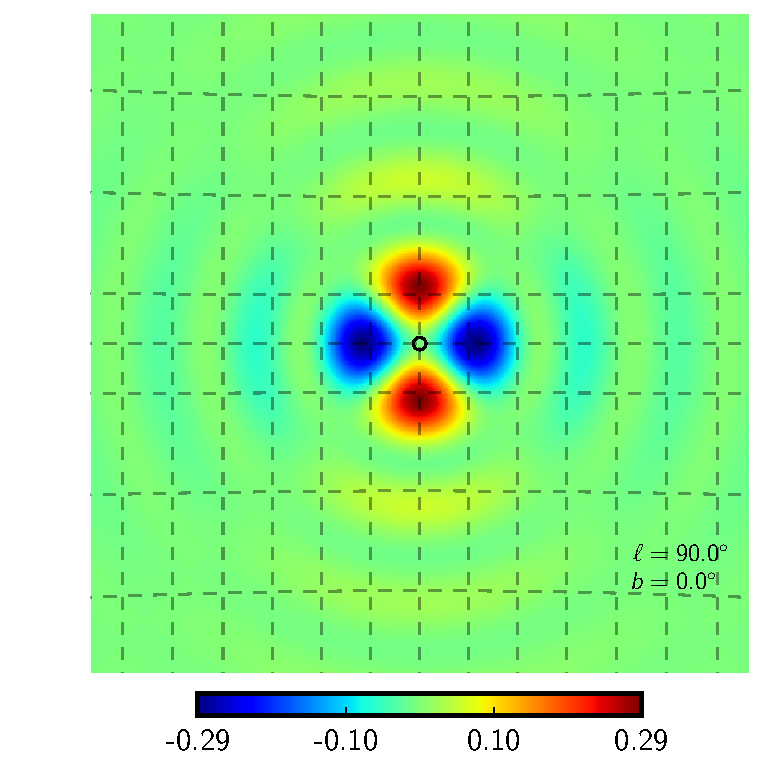
\includegraphics[width=0.16\columnwidth]{qu2eb_ker_r_lat0_lon90.pdf}}\hspace{-2mm}
\subfigure[$\mathcal{M}_i$]{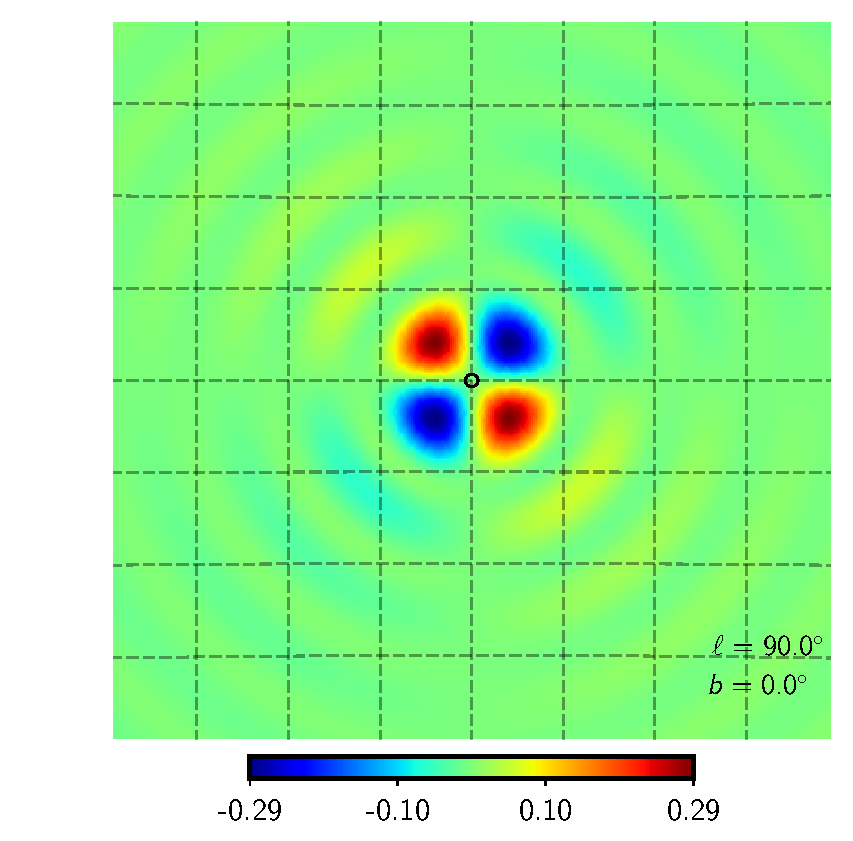
\includegraphics[width=0.16\columnwidth]{qu2eb_ker_i_lat0_lon90.pdf}}\hspace{-2mm}
\subfigure[$\mathcal{D}_r$]{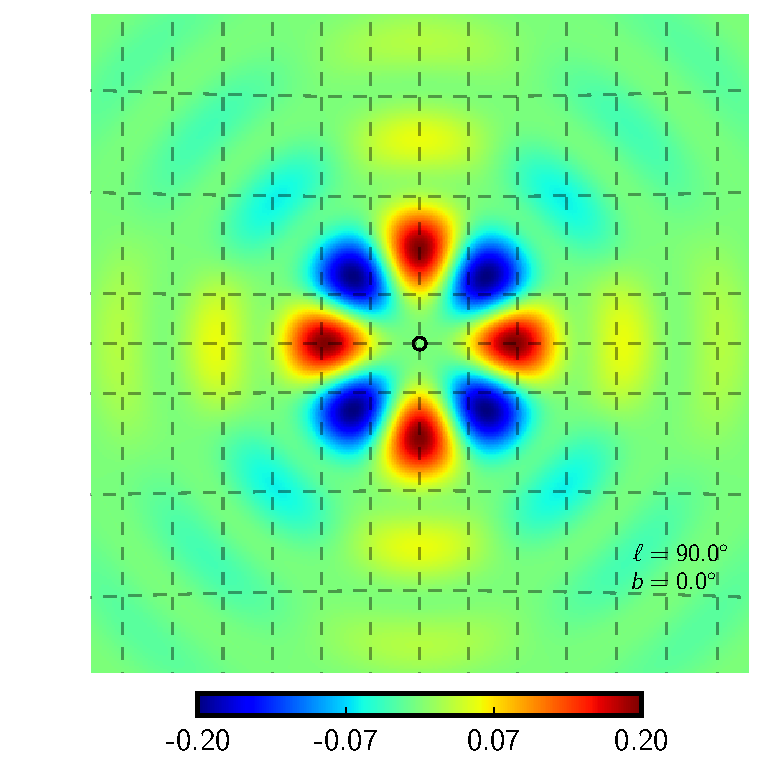
\includegraphics[width=0.16\columnwidth]{qu2ebqu_ker_r_lat0_lon90.pdf}}\hspace{-2mm}
\subfigure[$\mathcal{D}_i$]{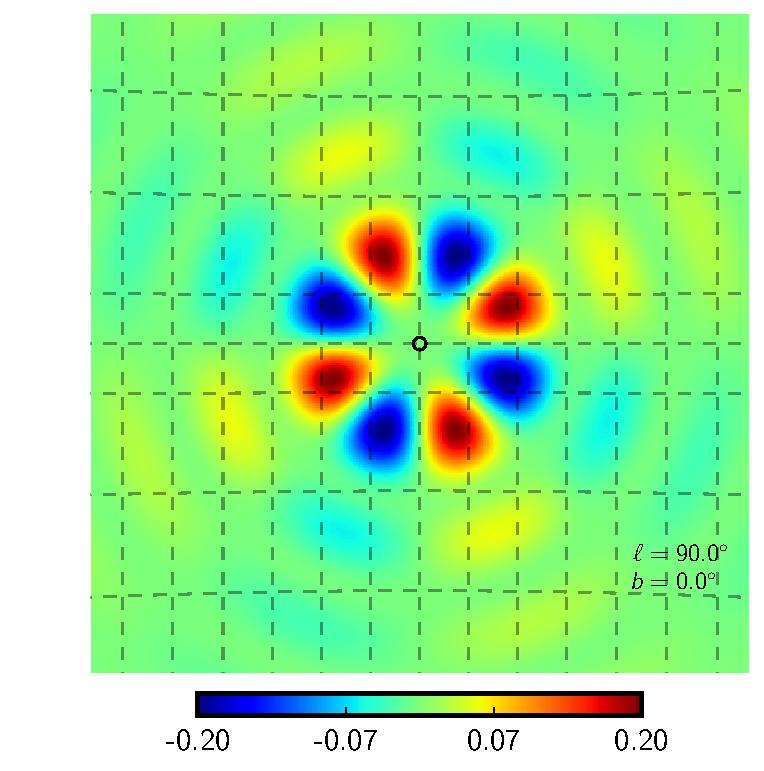
\includegraphics[width=0.16\columnwidth]{qu2ebqu_ker_i_lat0_lon90.pdf}}\hspace{-2mm}
\subfigure[$\mathcal{I}_r$]{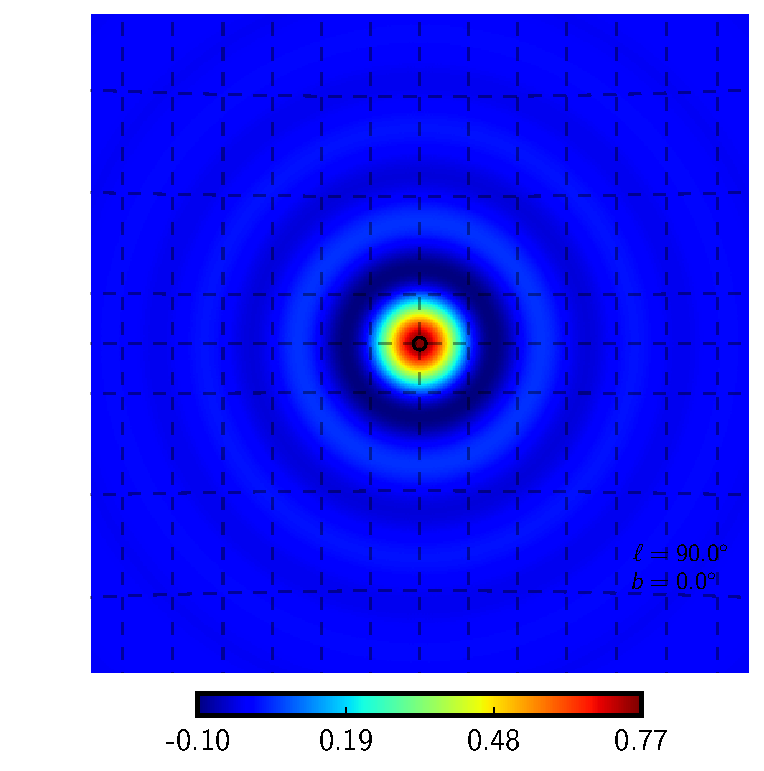
\includegraphics[width=0.16\columnwidth]{I_ker_r_lat0_lon90.pdf}}\hspace{-2mm}
\subfigure[$\mathcal{I}_i$]{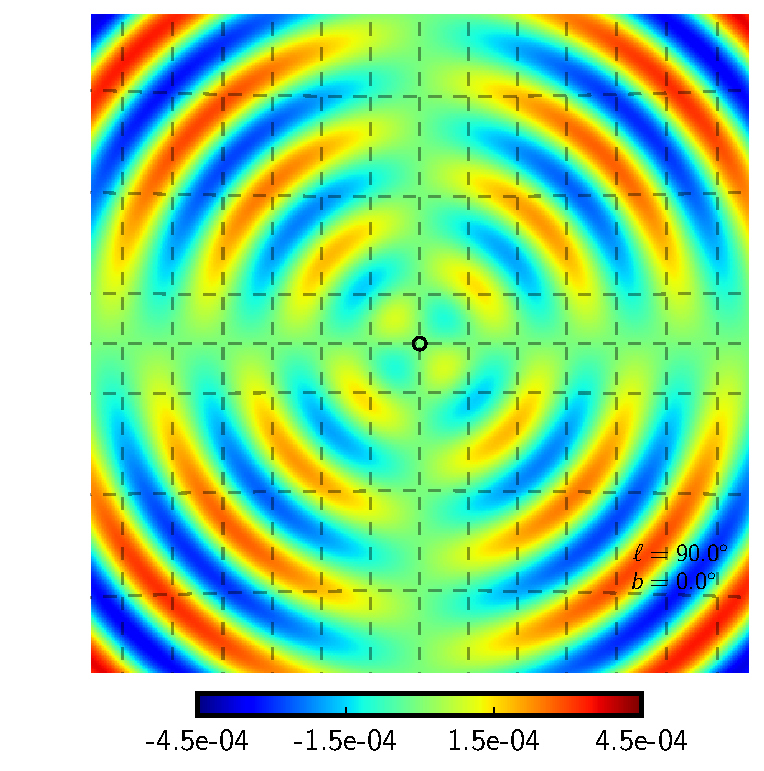
\includegraphics[width=0.16\columnwidth]{I_ker_i_lat0_lon90.pdf}}
\caption{This panel of figure depicts the various parts of the convolution kernel, discussed in \sec{sec:real_space_operators}. These kernels have been evaluated with the band limit fixed at $\ell_{\rm max}=96$, however the functions have been sampled at an NSIDE=2048 resolution for visual appeal. The size of each panel is approximately $26^{\circ} \times 26^{\circ}$. The black circles denotes the position of the central pixel around which the convolution kernels have been evaluated and the black star marks the location of the north galactic pole. The five rows depict the kernels at different location on the sphere and the galactic coordinates of the central pixel from top to bottom rows are as follows $[b,\ell] = [0^{\circ},0^{\circ}], [87^{\circ},0^{\circ}], [87^{\circ},30^{\circ}], [80^{\circ},30^{\circ}], [0^{\circ},90^{\circ}]$.}
\label{fig:vis_kernel}
 \end{figure}
%
\revisit{Since its not easy to imagine how the Euler angles vary as a function of position of the central pixel, we evaluate and depict the kernel at different locations on the sphere, to give a sense of how these kernels vary across the sphere.}
The function $\mathcal{M}$ is nearly identical irrespective of changes in the galactic latitude and longitude of the central pixel. The only contrasting locations are the poles (i.e. $|b|=90^{\circ}$), where the functions $\mathcal{M}_r$ \& $\mathcal{M}_i$ are rotated by $45^{\circ}$  as compared to the respective functions evaluated at locations where $|b|\neq 90^{\circ}$. It is also important to note that these functions are not distorted when a part of the domain overlaps with the poles, as can be seen in the first four rows of \fig{fig:vis_kernel}. On the contrary, the function $\mathcal{D}$ varies significantly as a function of galactic latitude of the central pixel. It varies from having a two fold symmetry at the poles to having a four fold symmetry at the equator as seen in the middle two columns of \fig{fig:vis_kernel}. This transformation arises from the distortions induced in this function as parts of its domain passes the galactic poles.  The function $\mathcal{I}$ shows similar behavior, varying with latitude and being distorted in parts that overlap with the galactic poles. \revisit{This function, in the ideal case of no band limit would reduces to a delta function at the position of the central pixel ($\lim_{\ell_{\rm max} \to \infty}: \mathcal{I}_r \rightarrow \delta(\hat{n}_0 - \hat{n}'),~ \mathcal{I}_i \rightarrow 0$), \revisit{hints of which can be seen by comparing the amplitudes of the real and imaginary parts of this function in the last two columns of \fig{fig:vis_kernel}, especially close to the equator}. Since we invariably work with a specific band limit, both the real and imaginary parts of this functions make important finite non-zero contributions }. All the function are seen to be invariant under changes in longitude of the central pixel, the latitude being held fixed as can be seen by comparing the figures in the second (evaluated at $[b,\ell]=[87^{\circ},0^{\circ}]$) and third row (evaluated at $[b,\ell]=[87^{\circ},30^{\circ}]$) of \fig{fig:vis_kernel}, as one may have expected.

\section{Quantifying the non-locality of E \& B modes} \label{sec:radial_locality}
It is clear that the non-locality of the E and B modes is determined by the radial part of the convolution kernels. To quantify this non-locality as a function of the resolution of the experiment, we evaluate only the radial part of the convolution kernel for different values of the maximum multipole $\ell_{\rm max}$, while keeping the lowest multipole fixed at $\ell_{\rm min}=2$. The set of radial kernels so derived are plotted in \fig{fig:rad_ker_decay}. All the function have been normalized such that their global maxima is set to unity. Note that on increasing $\ell_{\rm max}$ the radial kernels fall appear to shift left, becoming insignificant relative  to their global maxima at progressively small angular distance $\beta$ from the central pixel. 
%
\begin{figure}[!t]
\centering
\subfigure[]{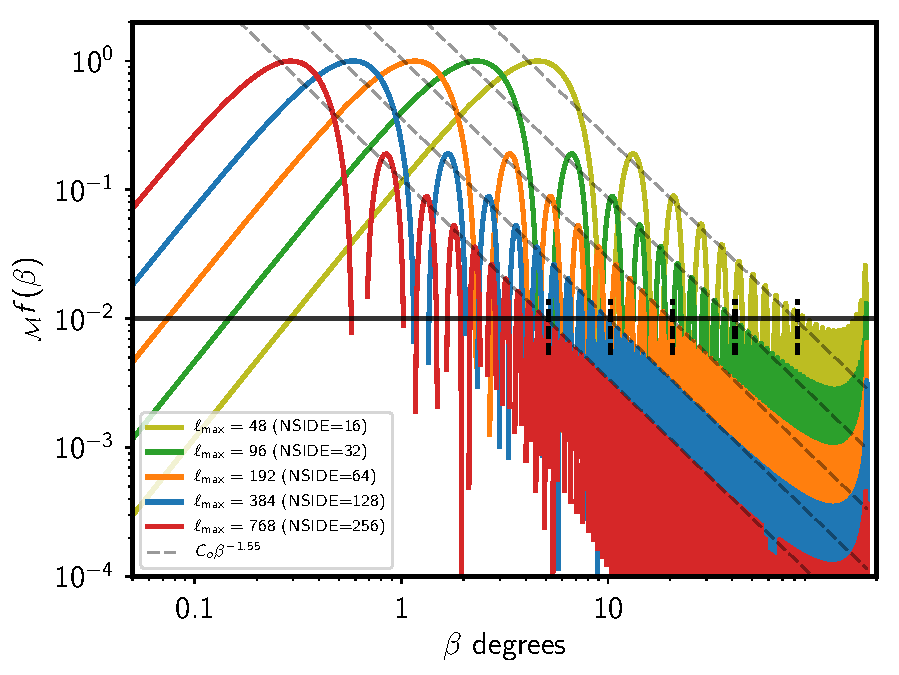
\includegraphics[width=1.0\columnwidth]{f_rad_ker_fn_of_ellmax.pdf}}
\subfigure[]{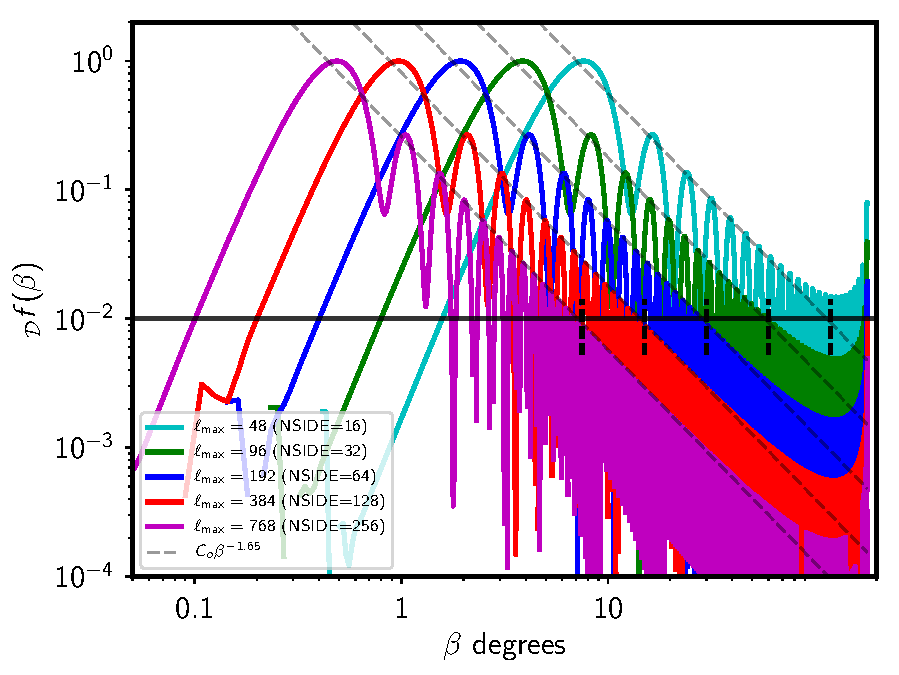
\includegraphics[width=0.48\columnwidth]{fp2_rad_ker_fn_of_ellmax.pdf}}
\subfigure[]{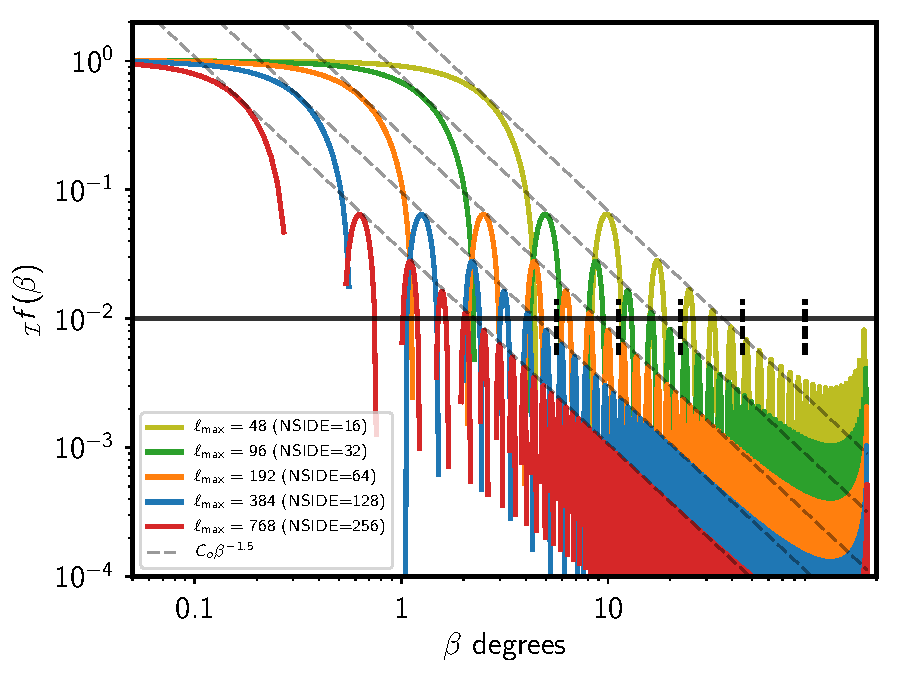
\includegraphics[width=0.48\columnwidth]{fm2_rad_ker_fn_of_ellmax.pdf}}
\caption{The top panel shows a plot of the radial kernels $f(\beta,\ell_{\rm min},\ell_{\rm max})$ while the bottom left and right panels show the radial functions ${}_{+2}f(\beta,\ell_{\rm min},\ell_{\rm max}) ~\&~ {}_{-2}f(\beta,\ell_{\rm min},\ell_{\rm max})$ respectively, for different $\ell_{\rm max}$ as indicated by the legends and fixed $\ell_{\rm min}=2$. The curves for each of these functions have been normalized such that the maximum of the curve is set to unity. The horizontal solid black line marks the location where the amplitude of the kernel falls below 1\% of its maximum. The slanted dashed black lines indicate a power law fit (by eye) to the envelope of the radial functions. While the envelopes for function $f(\beta)~\&~ {}_{-2}f(\beta)$ are fit well by the power law $\propto \beta^{-1.5}$, the envelope for the function ${}_{-2}f(\beta)$ is seen to have a slightly steeper fall off $\propto \beta^{-1.65}$.}
\label{fig:rad_ker_decay}
\end{figure}
%
We define the value of the abscissa at which the function $f(\beta,\ell_{\rm min},\ell_{\rm max})$ transits to being monotonously below 1\% of the maxima of the function as the non-locality parameter: $\beta_{o}$. We find that the following empirical relation: $\beta_o= {\rm max}(180,180 \frac{24}{\ell_{\rm max}})$ can predict quite accurately the value of the non-locality parameter for a given maximum multipole $\ell_{\rm max}$ and fixed $\ell_{\rm min}=2$. 

The envelope of the radial kernel $f(\beta,\ell_{\rm min},\ell_{\rm max})$ is observed to have a linear relation to the angular distance $\beta$ in log space as seen in \fig{fig:rad_ker_decay}, indicating a power law fall off. A fit by eye indicates that the envelope of the function is well represented by a fuction proportional to $\beta^{-1.5}$ in intermediate angular distance range. This is not valid in regions $\beta << \beta_o$ and $\beta >> \beta_o$, where the envelope of the function can be clearly seen to deviate from power law behavior (see \fig{fig:rad_ker_decay}).

\comment{There isn't too much of a discussion surrounding the function ${}_{\pm}f(\beta)$. What do you want to say about these functions?}

\comment{Do you want to comment on the telescoping behavior of these radial functions ? }
\section{Numerical implementation} \label{sec:numerical_implementation}

As discussed in \sec{sec:radial_locality}, the radial kernels decay ($\propto ~ \beta^{-1.5}$) as the distance from the central pixel increases, but they begin to increase on approaching the diametrically opposite position ($\beta \rightarrow \pi$)  as seen in \fig{fig:rad_ker_decay}). For a sufficiently high maximum multipole $\ell_{\rm max}$, the lowest multipole being fixed at $\ell_{\rm min}=2$, the maximum the radial kernel reaches near the vicity of the diametrically opposite end can be significantly smaller than global maxima of the radial kernel. This suggests that for sufficiently high resolution CMB maps (${\rm NSIDE} >32$), having high multipole information, it may suffice to restrict the convolution over the Stoke parameters Q \& U (to deduce either the scalar E \& B maps or pure Stokes Q \& U corresponding to either of the two scalar modes) to a local region around the central pixel. The locality of the region is quantified by the non-locality parameter $\beta_o$, which is a function of the maximum multipole accessible in the Stokes maps.

We have developed a Python script to evaluate these local convolution over Stokes Q \& U parameters. To evaluate the convolution kernel (\eq{eq:qu2eb_convolution}), we precompute the radial part of the kernel ( $f(\beta), {}_{+2}f(\beta) ~\&~ {}_{-2}f(\beta))$. Specifically, we use the python routine {\textit scipy.special.lpmn} to evaluate the associated Legendre polynomial functions, which are needed to evaluate the radial kernels. $f(\beta)$ is simply evaluated by calculating the multipole sum in \eq{eq:rad_ker_queb}. ${}_{+2}f(\beta) ~\&~ {}_{-2}f(\beta))$ are estimated by evaluating the sum in \eq{eq:f2_rad_ker}, where we take care to use the limiting forms of the functions ${}_{\pm 2}f_{\ell}(\beta)$ in the vicinity of $\beta=0,\pi$ as discussed in \app{sec:asymptotic_f}. As the next step, for each pixel on the Healpix map we get the pixel numbers of all the neighboring pixels lying within radius of $r_{\rm cutoff}$ from the central pixel using the Healpix routine {\textit query\_disc}. We then use the {\textit pix2ang} function of Healpix to get the angular coordinates of the central $(\theta_o,\phi_o)$ and its surrounding pixels $(\theta_i,\phi_i)$, which are then used to calculate the corresponding Euler angles using \eq{eq:fn_euler}. Given these  inputs we evaluate the convolution kernel as simple Reimann sums. We repeat this procedure for each pixel on the Healpix map. 

For the results presented in the following sub-sections we work with CMB maps at Healpix resolution of ${\rm NSIDE}=64$, unless specified otherwise. \revisit{We use the CMB spectra for some fiducial cosmology. This work  only deals with lensing B-mode spectra.} To understand the effects of restricting the convolution to a local neighbourhood, we evaluate these convolutions on discs with progressively smaller radii surrounding the central pixel.  Specifically the non-locality parameter for a NSIDE=64 map is $\beta_o=30^{\circ}$. We impose radial cutoffs of $r_{\rm cutoff}=[2\beta_0,\beta_o,0.5\beta_o,0.25\beta_o]$ with an apodization of 3 degrees having a cosine squared profiles on the edges of the discs. We also evaluate the corresponding maps using standard Healpix routines and use these as reference maps for this exercise. Note that the Healpix evaluations are in principle equivalent to carrying out the convolution over the full sphere (i.e. $\beta_o=\pi$).  We compare the spectra derived from all these maps to those derived from the reference maps to quantify the effect of the imposed radial cutoff on the convolution integrals.

%--------------------------------------------------------
%--------------------------------------------------------
\subsection{Constructing E \& B maps from local convolutions on Stokes Q \& U maps}

%
\begin{figure}[!h] 
\centering
\subfigure[E-mode Healpix]{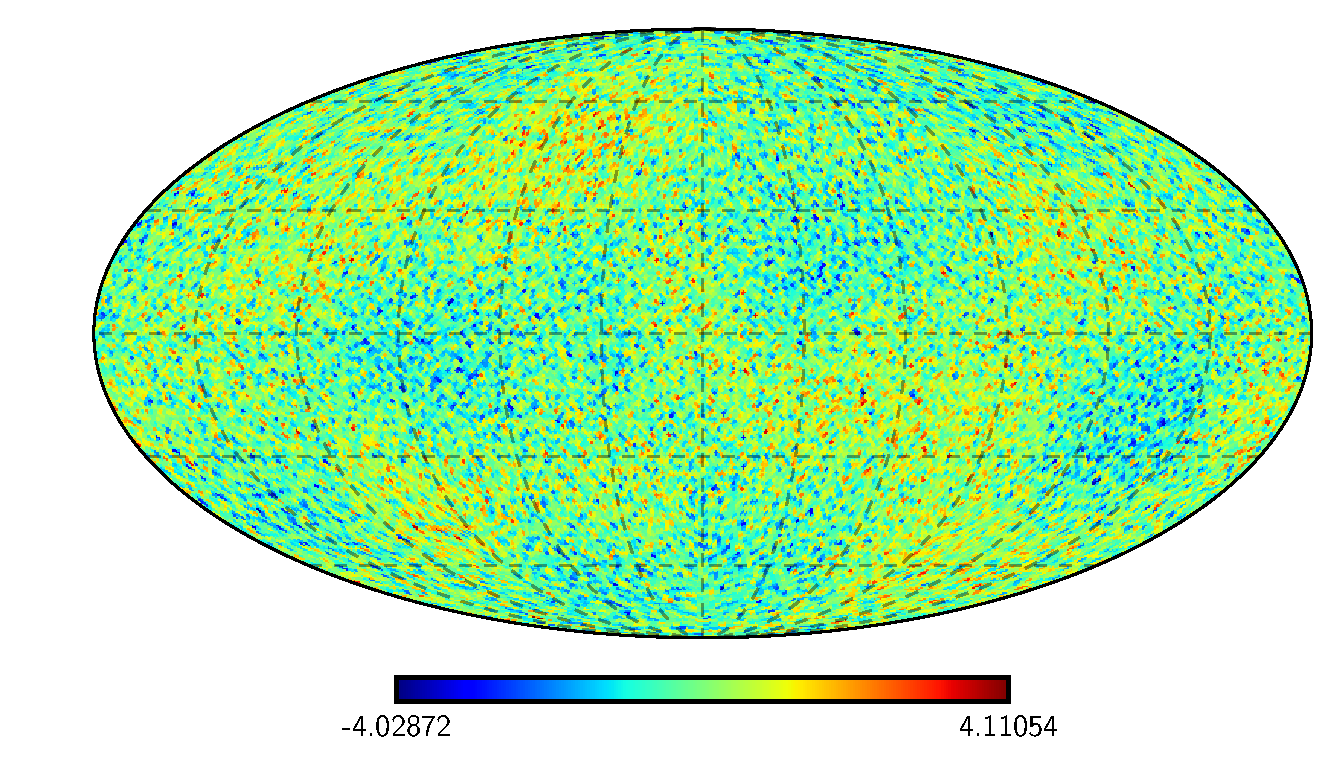
\includegraphics[width=0.31\columnwidth]{emap-healpix.pdf}}
\subfigure[E-mode local convolution]{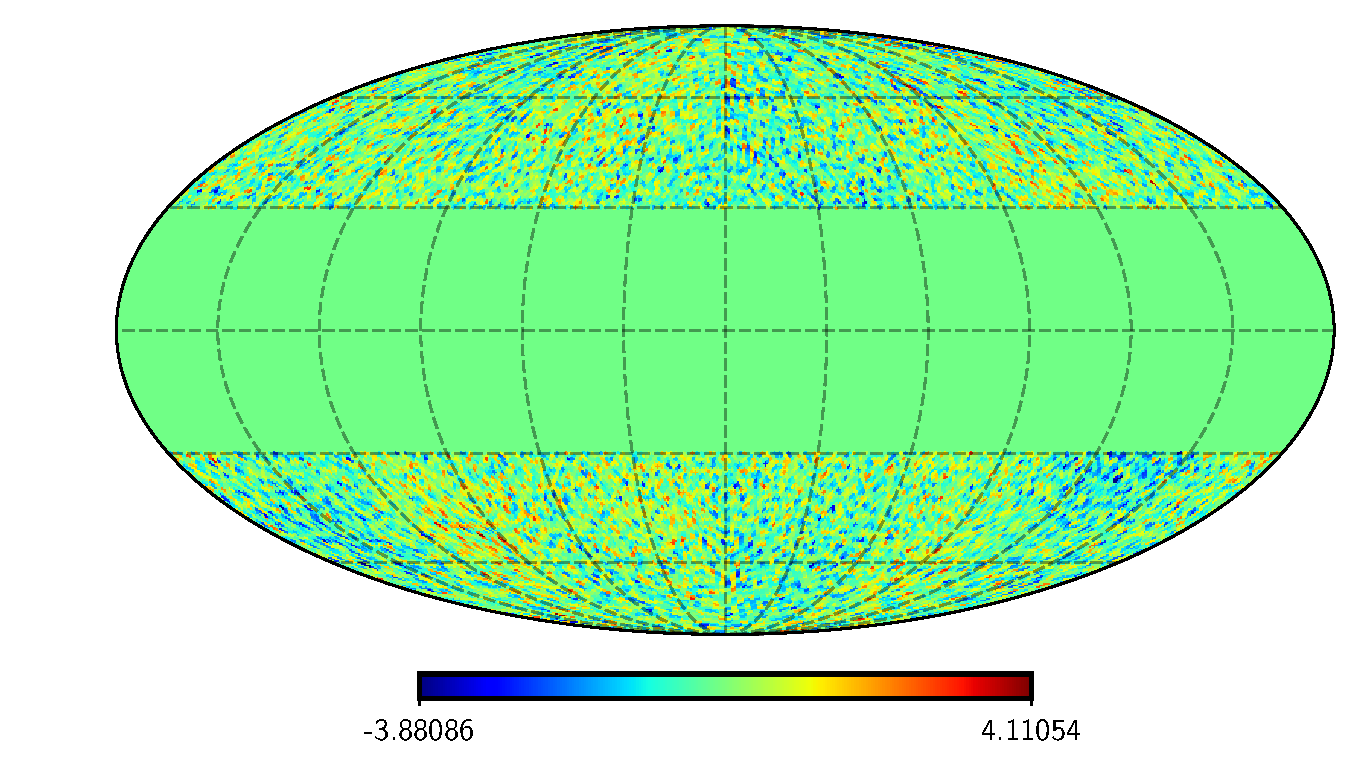
\includegraphics[width=0.31\columnwidth]{emap-2beta.pdf}}
\subfigure[Difference]{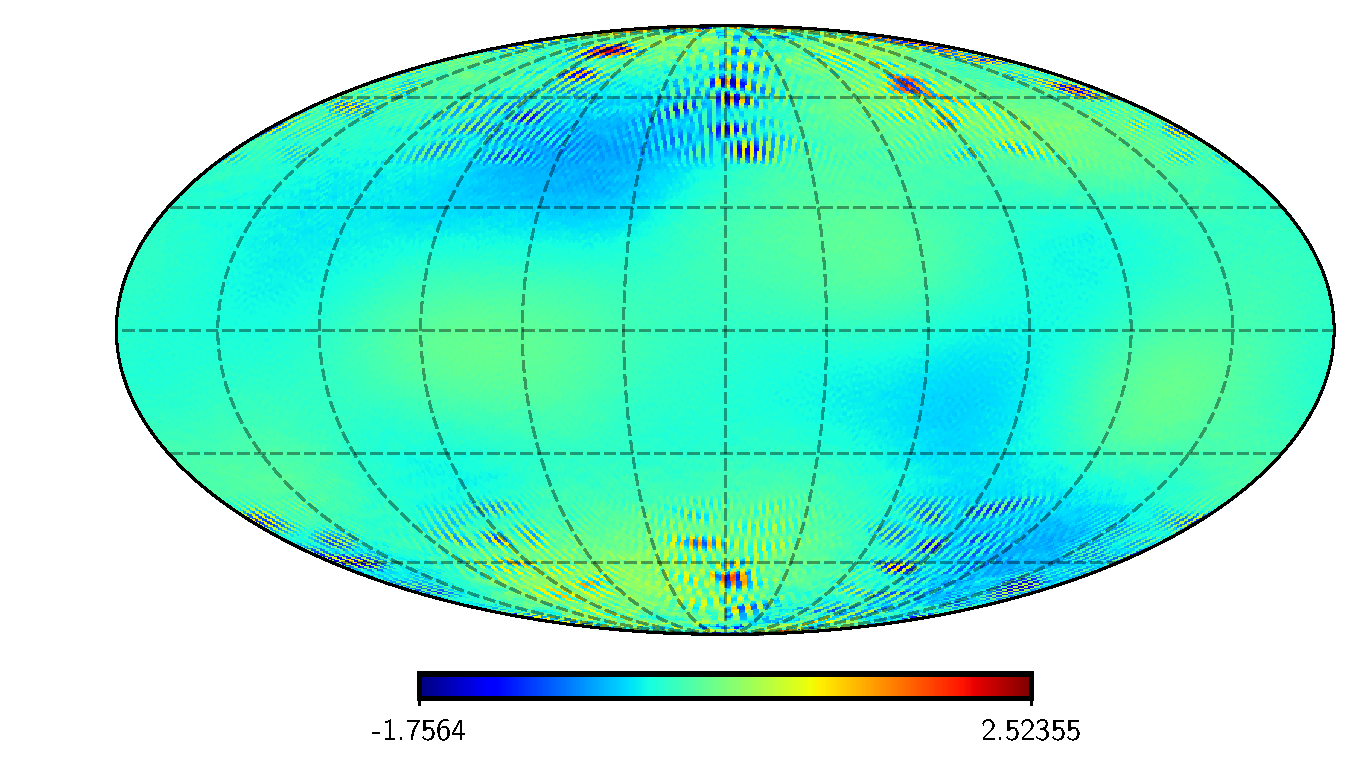
\includegraphics[width=0.31\columnwidth]{emap-diff.pdf}}
\subfigure[B-mode Healpix]{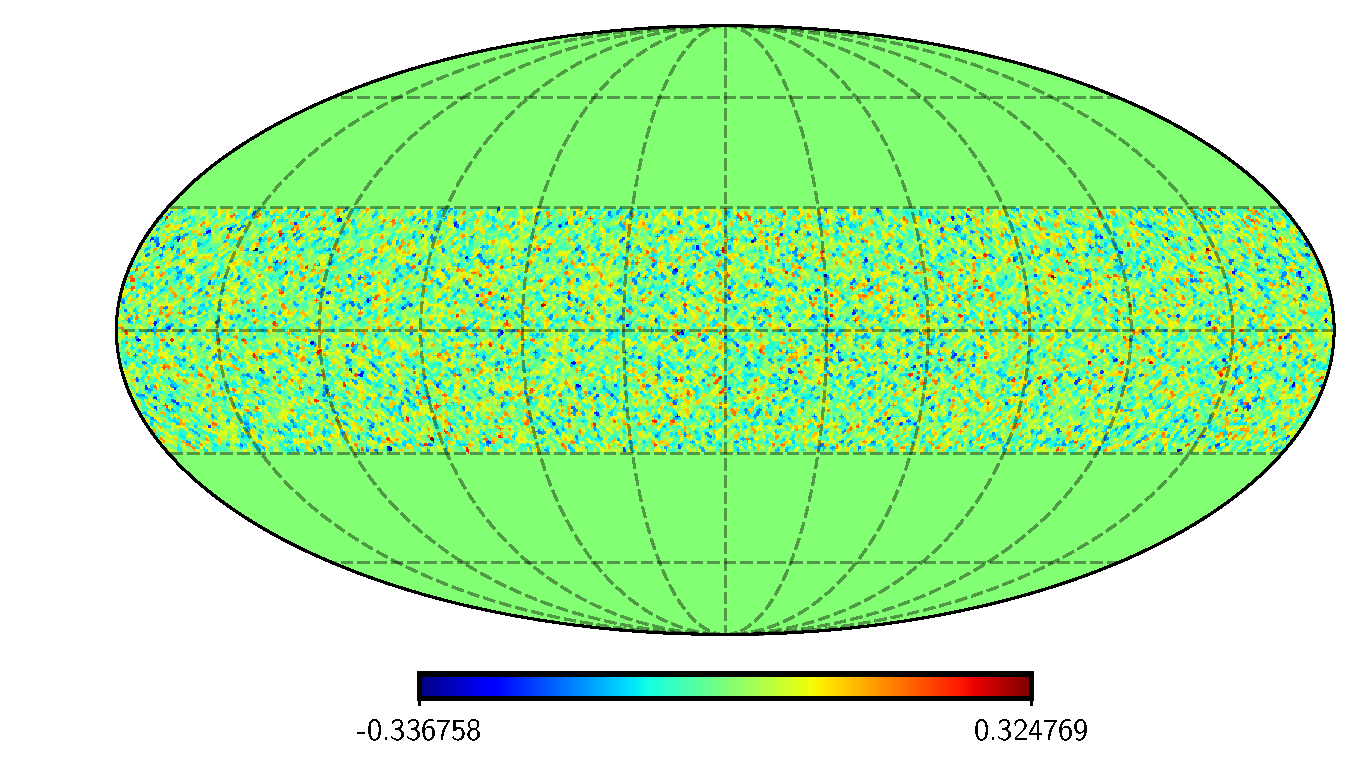
\includegraphics[width=0.31\columnwidth]{bmap-healpix.pdf}}
\subfigure[B-mode local convolution]{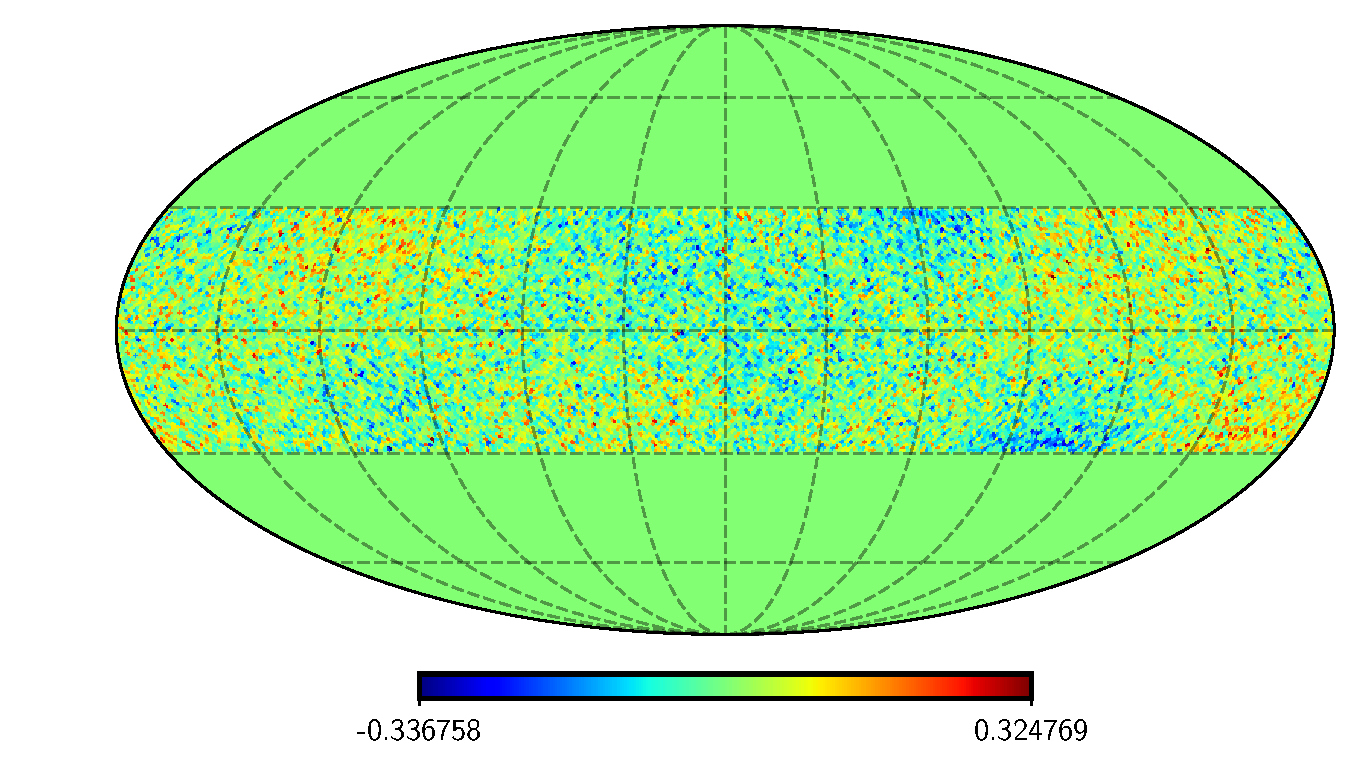
\includegraphics[width=0.31\columnwidth]{bmap-2beta.pdf}}
\subfigure[Difference]{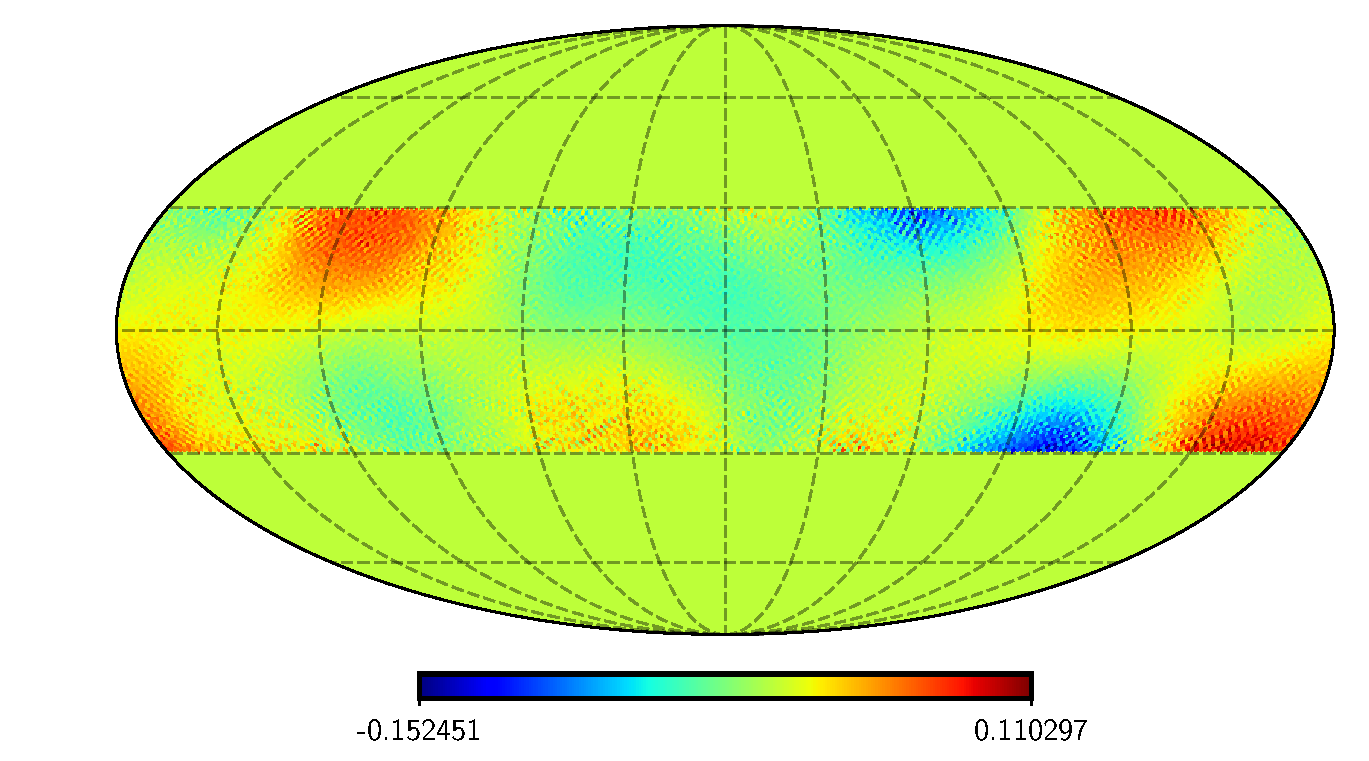
\includegraphics[width=0.31\columnwidth]{bmap-diff.pdf}}
\caption{{\textit Left:} Reference E \& B mode maps derived using Healpix. {\textit Middle:} E \& B mode maps derived using $r_{\rm cutoff}=2\beta_o$. {\textit Right:} Difference between the maps shown in the left and middle columns. Note that the differences maps are primarily due to differences in the recovery of large scale modes.}
\label{fig:eb-maps-compare}
\end{figure}
%
%
\begin{figure}[!h] 
\centering
\subfigure[]{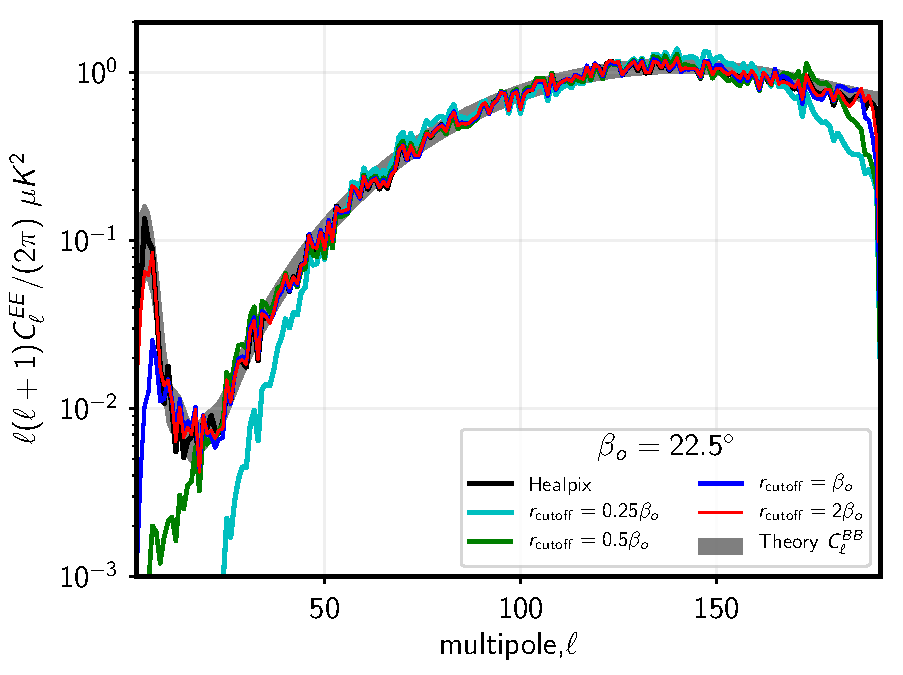
\includegraphics[width=0.49\columnwidth]{ee-spectrum-radial-cutoff.pdf}}
\subfigure[]{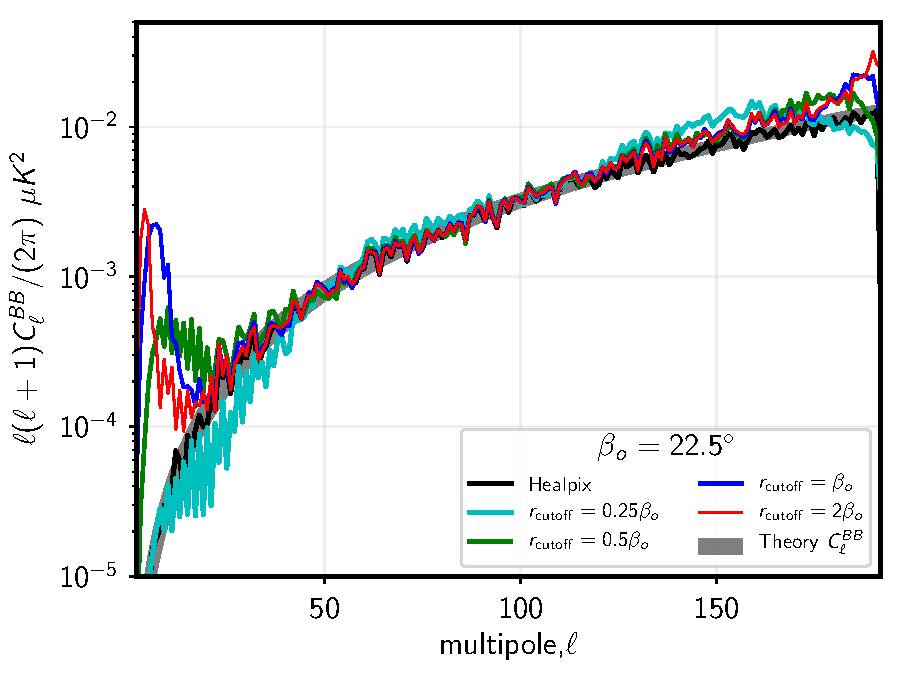
\includegraphics[width=0.49\columnwidth]{bb-spectrum-radial-cutoff.pdf}}
\subfigure[]{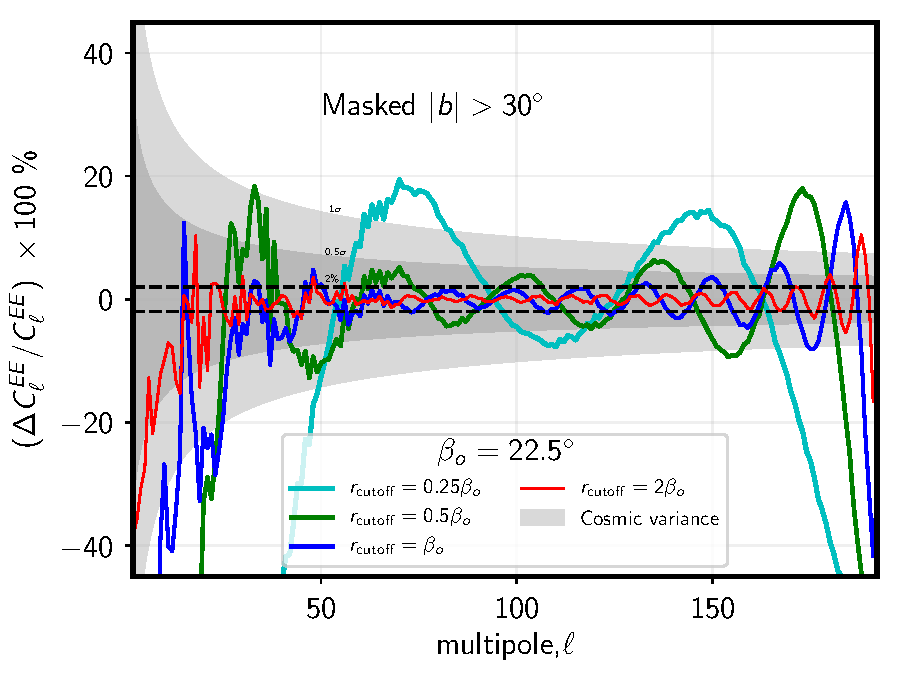
\includegraphics[width=0.49\columnwidth]{relative-percentage-err-ee-spectrum-radial-cutoff.pdf}}
\subfigure[]{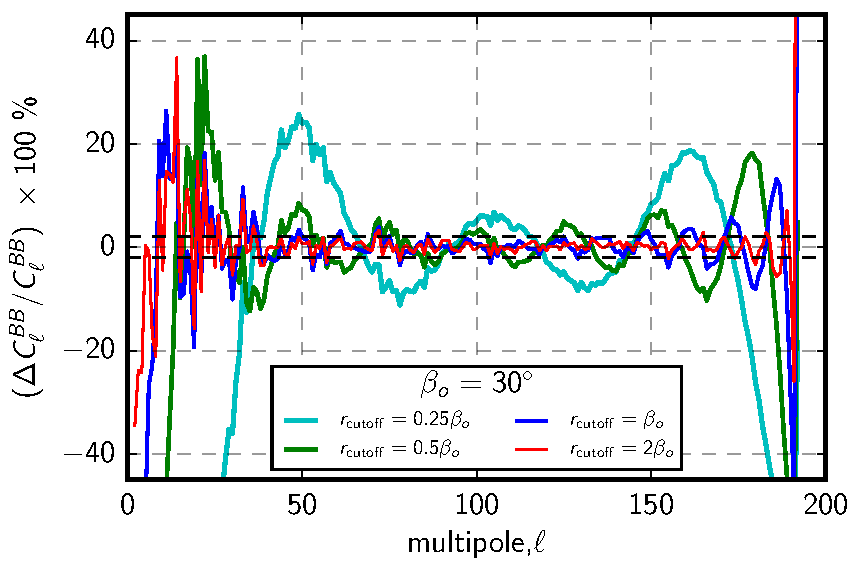
\includegraphics[width=0.49\columnwidth]{relative-percentage-err-bb-spectrum-radial-cutoff.pdf}}
\caption{}
\label{fig:eq-spectra_rad_cutoff}
\end{figure}
%
%--------------------------------------------------------
%--------------------------------------------------------
\subsection{Extracting Equ and Bqu maps}
%
\begin{figure}[!h] 
\centering
\subfigure[E-Q map Healpix]{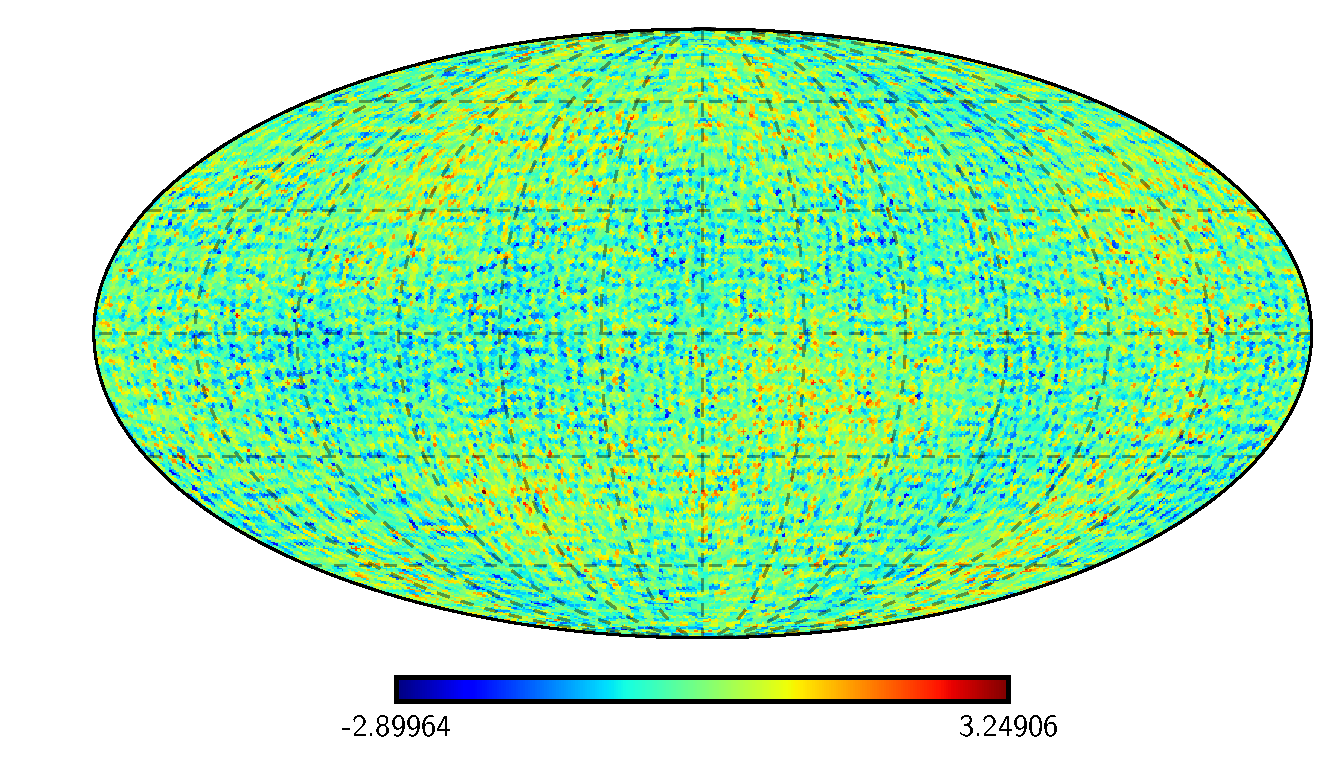
\includegraphics[width=0.31\columnwidth]{e-qmap-healpix.pdf}}
\subfigure[E-Q map local convolution]{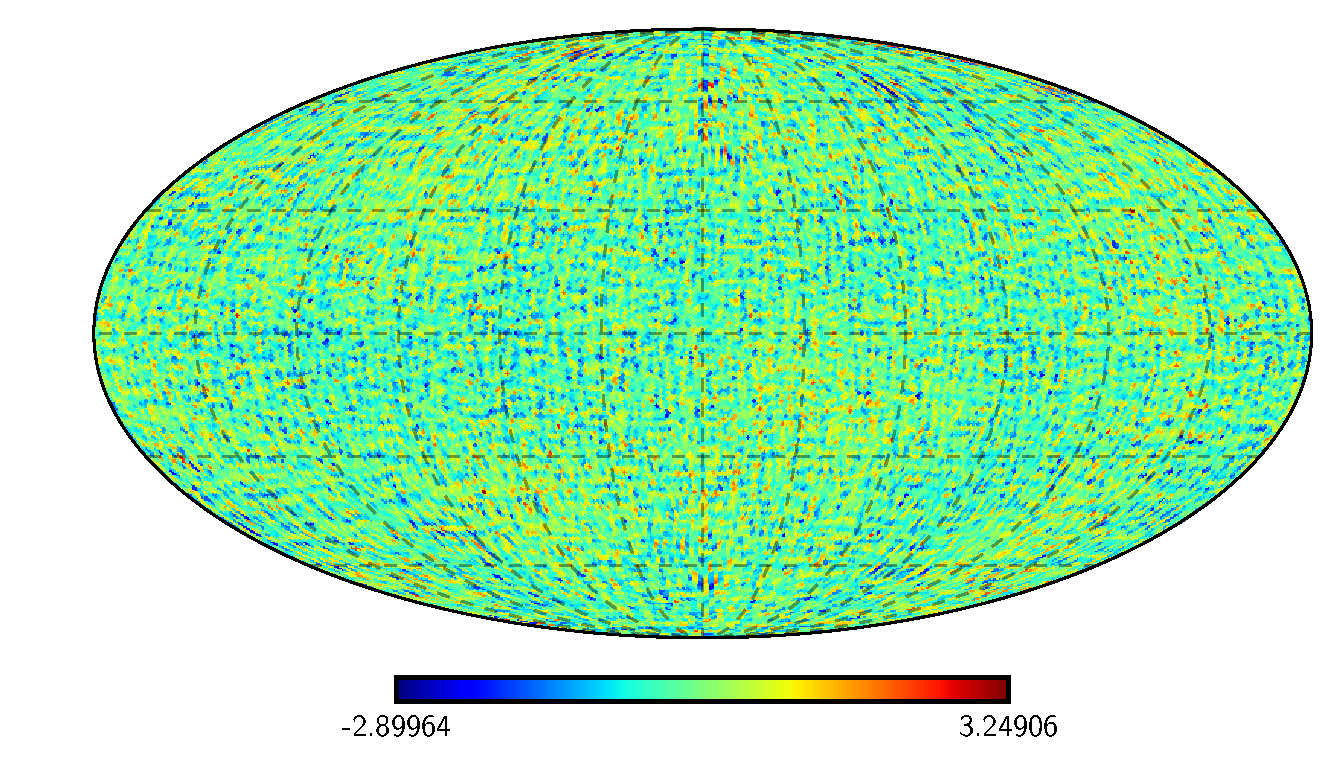
\includegraphics[width=0.31\columnwidth]{e-qmap-2beta.pdf}}
\subfigure[E-Q map difference]{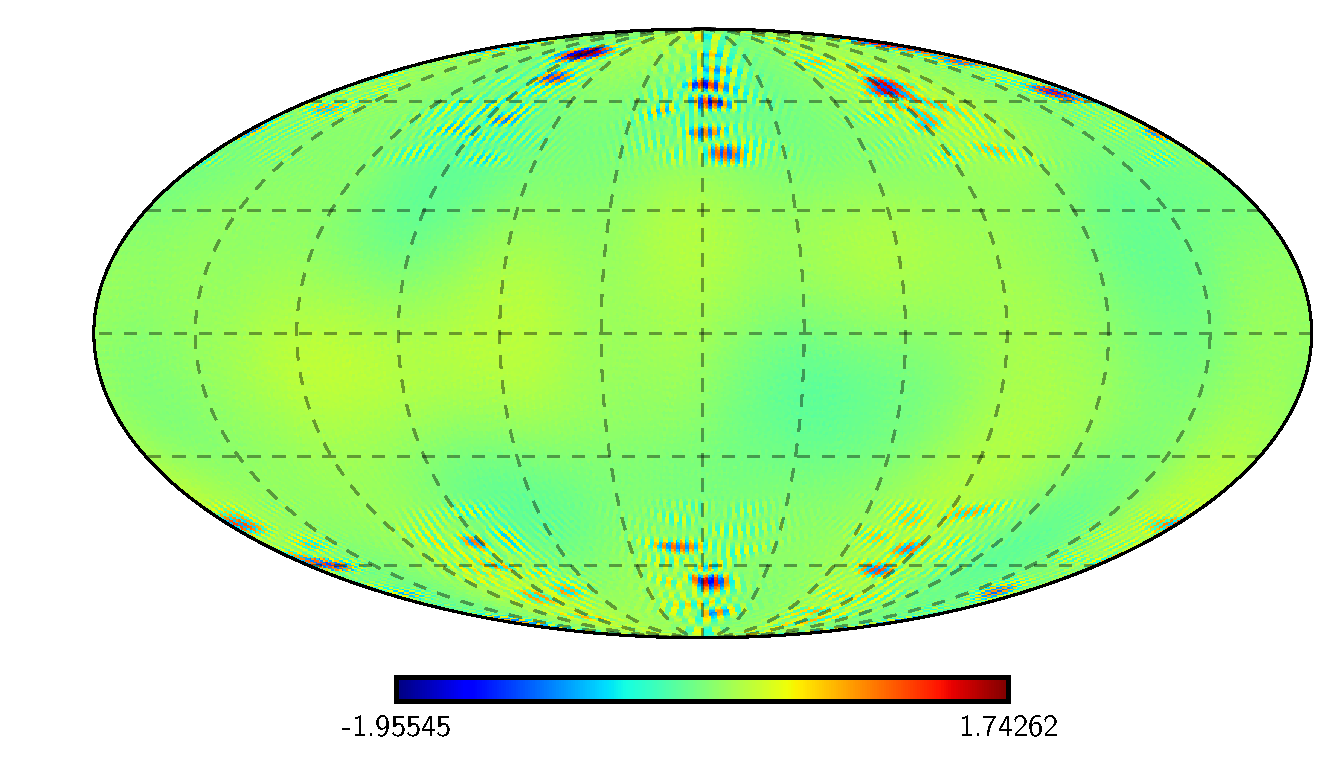
\includegraphics[width=0.31\columnwidth]{e-qmap-diff.pdf}}
\subfigure[E-U map Healpix]{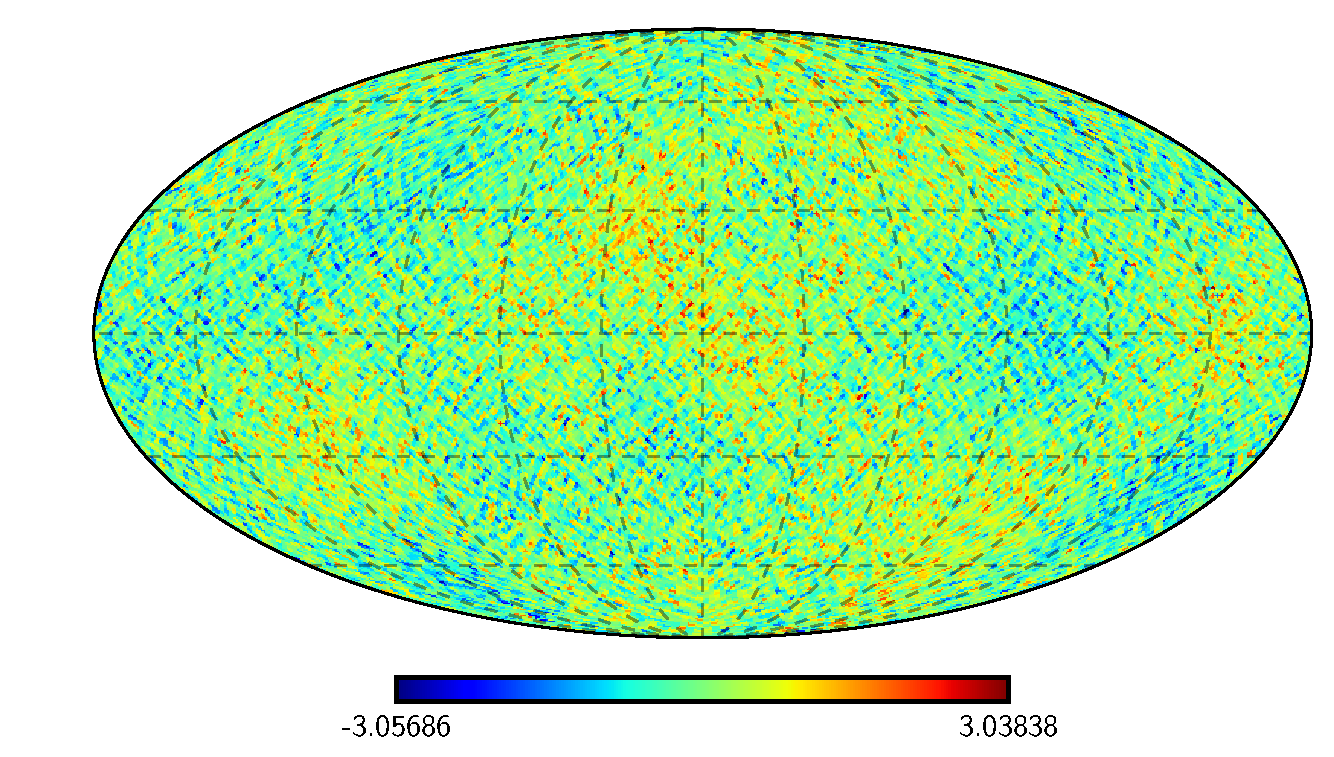
\includegraphics[width=0.31\columnwidth]{e-umap-healpix.pdf}}
\subfigure[E-U map local convolution]{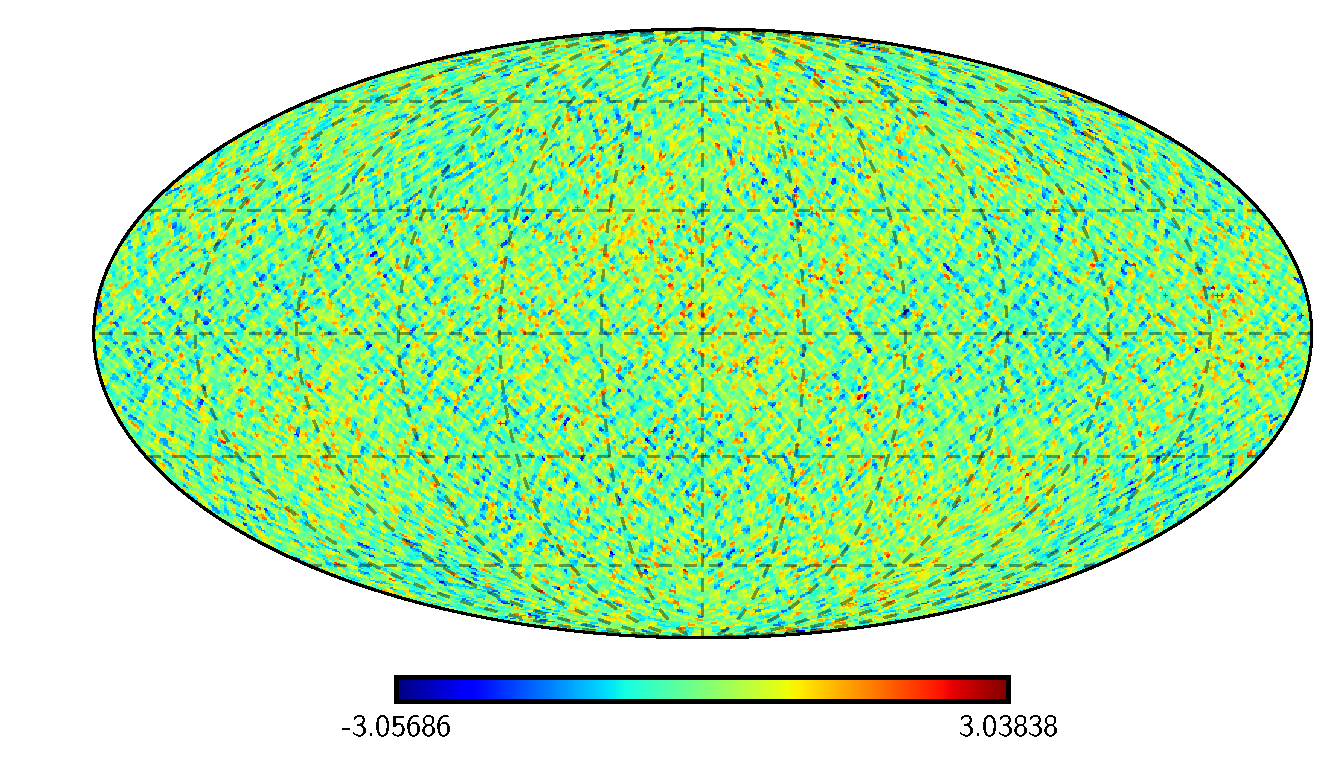
\includegraphics[width=0.31\columnwidth]{e-umap-2beta.pdf}}
\subfigure[E-U map difference]{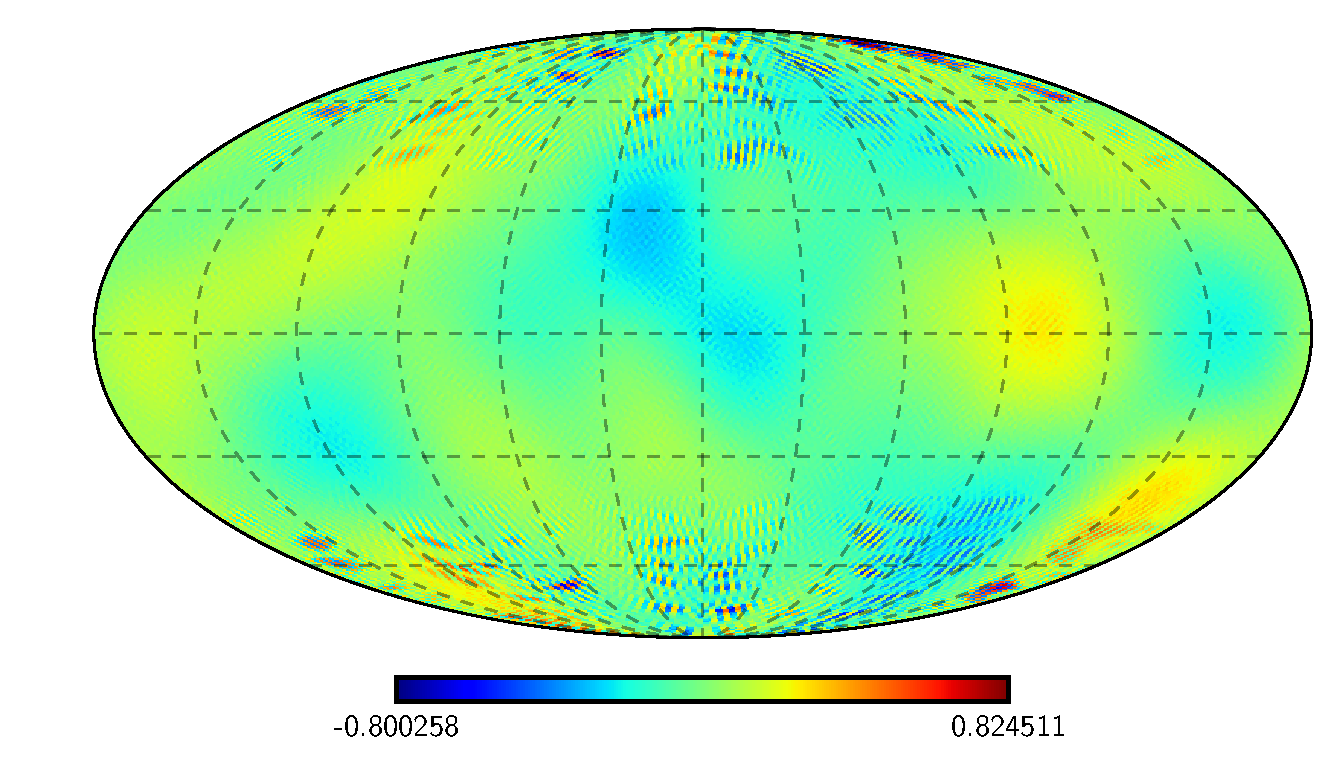
\includegraphics[width=0.31\columnwidth]{e-umap-diff.pdf}}

\subfigure[B-Q map Healpix]{\includegraphics[width=0.31\columnwidth]{b-qmap-healpix.pdf}}
\subfigure[B-Q map local convolution]{\includegraphics[width=0.31\columnwidth]{b-qmap-2beta.pdf}}
\subfigure[B-Q map difference]{\includegraphics[width=0.31\columnwidth]{b-qmap-diff.pdf}}
\subfigure[B-U map Healpix]{\includegraphics[width=0.31\columnwidth]{b-umap-healpix.pdf}}
\subfigure[B-U map local convolution]{\includegraphics[width=0.31\columnwidth]{b-umap-2beta.pdf}}
\subfigure[B-U map difference]{\includegraphics[width=0.31\columnwidth]{b-umap-diff.pdf}}
\caption{}
\label{fig:equ-bqu-maps-compare}
\end{figure}
%

%
\begin{figure}[!h] 
\centering
\subfigure[]{\includegraphics[width=0.49\columnwidth]{equ-spectra-radial-cutoff.pdf}}
\subfigure[]{\includegraphics[width=0.49\columnwidth]{bqu-spectra-radial-cutoff.pdf}}
\subfigure[]{\includegraphics[width=0.49\columnwidth]{relative-percentage-err-equ-e-spectrum-radial-cutoff.pdf}}
\subfigure[]{\includegraphics[width=0.49\columnwidth]{relative-percentage-err-bqu-b-spectrum-radial-cutoff.pdf}}
\caption{}
\label{fig:equ-bqu-spectra_rad_cutoff}
\end{figure}
%
%--------------------------------------------------------
%--------------------------------------------------------
\subsection{Scaling and future prospects}
%
\begin{figure}[!h] 
\centering
\subfigure[]{\includegraphics[width=0.8\columnwidth]{number_of_disc_pixels.pdf}}
\caption{The red dashed curve depicts the how $\beta_o$ changes as a function of the Healpix resolution parameter Nside assuming that the maximum multipole accessible in the map is given by $\ell_{\rm max} = 3 * Nside$. The blue solid curve depicts the number of surrounding pixel that will need to be accessed to carry out the convolution on Stokes Q \& U maps to infer the value of the scalar fields E \& B at the central pixel.}
\label{fig:disc_rad_healpix_numpix}
\end{figure}
%
%--------------------------------------------------------
%--------------------------------------------------------
\subsection{Application of Planck 353 Ghz polarization maps}
%
\begin{figure}[!h] 
\centering
\subfigure[]{\includegraphics[width=0.49\columnwidth]{353ghz-e-mode-healpix.pdf}}
\subfigure[]{\includegraphics[width=0.49\columnwidth]{353ghz-e-mode-real-space-disc8apo3.pdf}}
\subfigure[]{\includegraphics[width=0.49\columnwidth]{353ghz-b-mode-healpix.pdf}}
\subfigure[]{\includegraphics[width=0.49\columnwidth]{353ghz-b-mode-real-space-disc8apo3.pdf}}
\caption{}
\label{fig:353ghz-eb-maps}
\end{figure}
%
\section{Discussion}\label{sec:discussion}
\begin{itemize}
\item We have derived the real space kernels for translating Stokes parameters Q \& U to scalars E \& B and vice versa. We have also derived real space kernels which allow for direct separation of Stokes Q \& U parameters without having to first evaluate the scalar field E \& B.

\item These kernels quantify the non-locality of the E and B fields. We have introduced the non-locatity parameter $\beta_0$ which provides a quantitative measure of the non-locality of these fields.  

\item Studying these real space kernels reveals that its the radial part of the kernel which knows about the band limit of the experiment. Motivation for defining radially compact kernels. We have demonstrated that using the radially compact kernels does not bias the spectral information on intermediate angular scales.

\item Small field experiments like BICEP, implicitly implement such radial cut offs due to limited survey area. 


\item Using in conjunction with FEBECOP \cite{febecop} like schemes to directly infer E and B mode maps from raw maps.

\item \textit{Mask leakages} can be understood as arising from improper sine quadrupole and cosine quadrupole transforms on rings with holes in them due to masking. For the global mask (no point sources), by using a radially compact kernel with some $\beta_0$, the pixels which are at a angular distance $\beta_0$ from the edges of the mask have unbiased estimates of the scalar fields E and B.

\end{itemize}
%
%The width of the $\beta$ kernel can be used as an indicator of the width of mask apodization. One may also use the width of the $\beta$ kernel to throw away the regions of the sky close to the edges of the mask. Mask apodization techniques should fail at low Nside. The width of the $\beta$ kernel makes transparent why the E to B leakage issues are only relevant close to the edges of the mask.